\documentclass[sigplan, 10pt, nonacm]{acmart}
\usepackage[moderate]{savetrees}

\newcommand{\alek}[1]{\textcolor{red}{#1}}

\usepackage{booktabs} % For formal tables


% Copyright
%\setcopyright{none}
%\setcopyright{acmcopyright}
%\setcopyright{acmlicensed}
\setcopyright{rightsretained}
%\setcopyright{usgov}
%\setcopyright{usgovmixed}
%\setcopyright{cagov}
%\setcopyright{cagovmixed}


% DOI
\acmDOI{10.475/123_4}

% ISBN
\acmISBN{123-4567-24-567/08/06}

%Conference
%% \acmConference[APOCS '20]{}{January 2020}{Salt Lake City, UT, USA}
%% \acmYear{2019}
%% \copyrightyear{2019}


\acmArticle{4}
\acmPrice{15.00}

\usepackage{mathtools}
\newcommand{\defeq}{\vcentcolon=}
\DeclarePairedDelimiter{\paren}{(}{)}

\usepackage{enumitem}
\usepackage{subcaption}

\usepackage{tikz,pgfplots}
\usepackage{etoolbox}
%% This makes the colors annoyingly bright, but at least they're easy to distinguish.
\pgfplotsset{
  every  tick/.style={red,}, minor x tick num=1,
  cycle list={teal,every mark/.append style={fill=teal!80!black},mark=*\\%
orange,every mark/.append style={fill=orange!80!black},mark=square*\\%
cyan!60!black,every mark/.append style={fill=cyan!80!black},mark=otimes*\\%
red!70!white,mark=star\\%
lime!80!black,every mark/.append style={fill=lime},mark=diamond*\\%
red,densely dashed,every mark/.append style={solid,fill=red!80!black},mark=*\\%
yellow!60!black,densely dashed,
every mark/.append style={solid,fill=yellow!80!black},mark=square*\\%
black,every mark/.append style={solid,fill=gray},mark=otimes*\\%
blue,densely dashed,mark=star,every mark/.append style=solid\\%
red,densely dashed,every mark/.append style={solid,fill=red!80!black},mark=diamond*\\%
}
}

%% Issues: One }; missing in bandwidth table by default
%% Same issue appears multiple times in sort table

\def \CILKserialbaseline {3932.2}
\def \CILKblocksize {64}
\def \CILKnumtrials {5}
\def \CILKinputsize {1073741824}
\def \CILKtable {
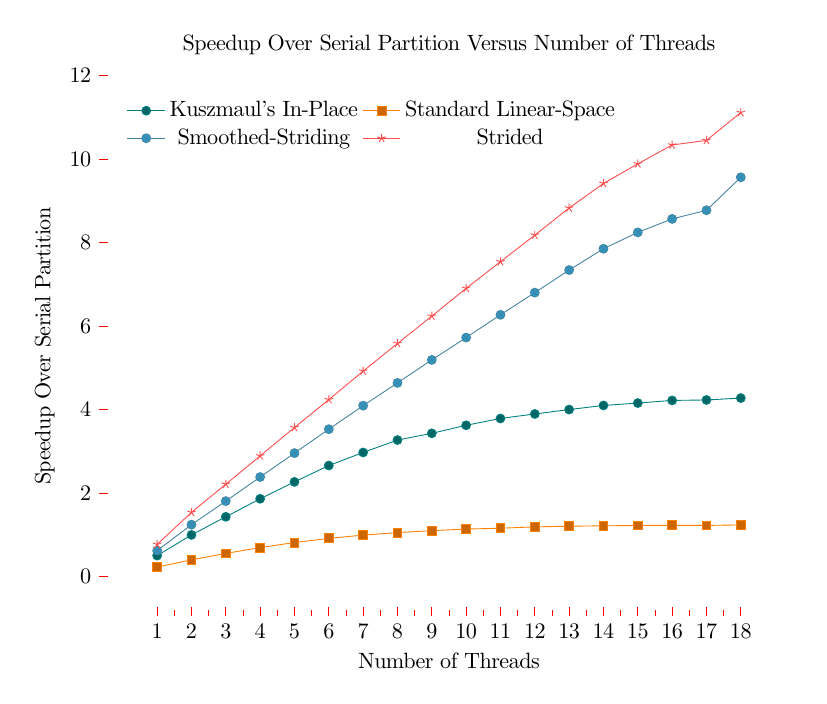
\begin{tikzpicture}[scale = .8]
\begin{axis}[
width = 5 in,
height = 4in,
title={Speedup Over Serial Partition Versus Number of Threads},
xtick pos=left,
ytick pos=left,
legend style={draw=none},
axis line style = { draw = none },
legend pos= north west,
xtick = data,
xlabel={Number of Threads},
ylabel={Speedup Over Serial Partition},
ymax = 12,
legend columns = 2,
scatter/classes=%
{a={mark=o,draw=blue}}]
%% In-Place
\addplot coordinates {( 1, 0.499048) ( 2, 0.995494) ( 3, 1.42948) ( 4, 1.86113) ( 5, 2.26614) ( 6, 2.65797) ( 7, 2.97174) ( 8, 3.26921) ( 9, 3.43004) ( 10, 3.62281) ( 11, 3.78679) ( 12, 3.89481) ( 13, 4.0002) ( 14, 4.0986) ( 15, 4.15578) ( 16, 4.2191) ( 17, 4.22999) ( 18, 4.27599) };
%% In-Place Prefix-Sum
% \addplot coordinates {( 1, 0.35092) ( 2, 0.636608) ( 3, 0.894292) ( 4, 1.11755) ( 5, 1.32674) ( 6, 1.5096) ( 7, 1.65121) ( 8, 1.77494) ( 9, 1.88432) ( 10, 1.97837) ( 11, 2.0581) ( 12, 2.11591) ( 13, 2.15699) ( 14, 2.18845) ( 15, 2.21159) ( 16, 2.21657) ( 17, 2.20736) ( 18, 2.21557) };
%% Out-of-Place
\addplot coordinates {( 1, 0.223968) ( 2, 0.398625) ( 3, 0.551717) ( 4, 0.691607) ( 5, 0.812203) ( 6, 0.912936) ( 7, 0.990429) ( 8, 1.05055) ( 9, 1.09777) ( 10, 1.13562) ( 11, 1.15517) ( 12, 1.18848) ( 13, 1.20383) ( 14, 1.21364) ( 15, 1.22103) ( 16, 1.22575) ( 17, 1.22285) ( 18, 1.23444) };
%% %% High-Span
%% \addplot coordinates {( 1, 0.796443) ( 2, 1.58021) ( 3, 2.21882) ( 4, 2.93667) ( 5, 3.32899) ( 6, 3.80217) ( 7, 4.3662) ( 8, 4.93375) ( 9, 5.09881) ( 10, 5.42822) ( 11, 5.75051) ( 12, 6.01806) ( 13, 6.37103) ( 14, 6.57999) ( 15, 6.72631) ( 16, 6.95718) ( 17, 7.06722) ( 18, 7.34442) };
%% Cache-Friendly
\addplot coordinates {( 1, 0.619888) ( 2, 1.24099) ( 3, 1.80558) ( 4, 2.38286) ( 5, 2.95654) ( 6, 3.52917) ( 7, 4.09348) ( 8, 4.63922) ( 9, 5.19034) ( 10, 5.72539) ( 11, 6.27145) ( 12, 6.80311) ( 13, 7.34442) ( 14, 7.85497) ( 15, 8.24706) ( 16, 8.57062) ( 17, 8.77723) ( 18, 9.5674) };
%% Strided
\addplot coordinates {( 1, 0.767408) ( 2, 1.5359) ( 3, 2.21084) ( 4, 2.89005) ( 5, 3.56954) ( 6, 4.2382) ( 7, 4.9214) ( 8, 5.58393) ( 9, 6.23961) ( 10, 6.90587) ( 11, 7.54451) ( 12, 8.18186) ( 13, 8.83243) ( 14, 9.4207) ( 15, 9.88984) ( 16, 10.3425) ( 17, 10.4524) ( 18, 11.1205) };
\legend{Kuszmaul's In-Place, Standard Linear-Space, Smoothed-Striding, Strided} %% Low-Space, Med-Space, High-Space, Smoothed-Striding, Strided 
\end{axis}
\end{tikzpicture}
}
\def \partitionbandwidthboundserialbaseline {3933.6}
\def \partitionbandwidthboundblocksize {64}
\def \partitionbandwidthboundnumtrials {5}
\def \partitionbandwidthboundinputsize {1073741824}
\def \partitionbandwidthboundtable {
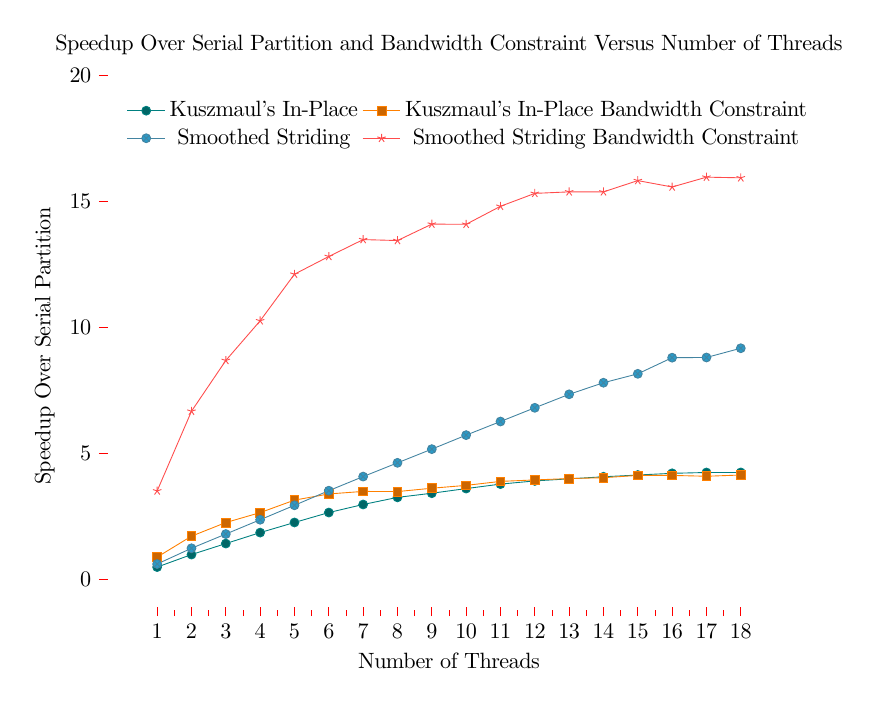
\begin{tikzpicture}[scale = .8]
\begin{axis}[
width = 5 in,
height = 4in,
title={Speedup Over Serial Partition and Bandwidth Constraint Versus Number of Threads},
xtick pos=left,
ytick pos=left,
legend style={draw=none},
axis line style = { draw = none },
legend pos= north west,
xtick = data,
xlabel={Number of Threads},
ylabel={Speedup Over Serial Partition},
ymax = 20,
legend columns = 2,
scatter/classes=%
{a={mark=o,draw=blue}}]
%% In-Place
\addplot coordinates {( 1, 0.499378) ( 2, 0.995949) ( 3, 1.4328) ( 4, 1.86816) ( 5, 2.26982) ( 6, 2.66432) ( 7, 2.98407) ( 8, 3.26602) ( 9, 3.43066) ( 10, 3.61544) ( 11, 3.79325) ( 12, 3.91949) ( 13, 4.00244) ( 14, 4.08389) ( 15, 4.15375) ( 16, 4.22151) ( 17, 4.25438) ( 18, 4.25622) };
%% Low-Space Bandwidth Bound
\addplot coordinates {(1, 0.894939)(2, 1.72634)(3, 2.26699)(4, 2.66131)(5, 3.15777)(6, 3.4024)(7, 3.50312)(8, 3.49686)(9, 3.62955)(10, 3.74294)(11, 3.90093)(12, 3.9593)(13, 4.0131)(14, 4.04714)(15, 4.13799)(16, 4.13782)(17, 4.10515)(18, 4.15355)};
%% high span
%% \addplot coordinates {( 1, 0.812828) ( 2, 1.61997) ( 3, 2.22137) ( 4, 2.95626) ( 5, 3.33582) ( 6, 3.80352) ( 7, 4.36001) ( 8, 5.10062) ( 9, 5.11521) ( 10, 5.44217) ( 11, 5.74752) ( 12, 6.07787) ( 13, 6.41278) ( 14, 6.63787) ( 15, 6.68752) ( 16, 6.79848) ( 17, 7.10549) ( 18, 7.26292) };
%% %% High-Span Bandwidth Bound
%% \addplot coordinates {(1, 1.75849)(2, 3.34185)(3, 4.35383)(4, 5.15739)(5, 5.9788)(6, 6.31621)(7, 6.76074)(8, 6.76348)(9, 6.99773)(10, 7.10173)(11, 7.39957)(12, 7.51437)(13, 7.7436)(14, 7.76191)(15, 7.89966)(16, 7.87403)(17, 7.94484)(18, 8.05483)}; %% cache friendly
\addplot coordinates {( 1, 0.62101) ( 2, 1.24639) ( 3, 1.81072) ( 4, 2.37852) ( 5, 2.95182) ( 6, 3.53233) ( 7, 4.09153) ( 8, 4.63759) ( 9, 5.18124) ( 10, 5.73746) ( 11, 6.27769) ( 12, 6.82206) ( 13, 7.35802) ( 14, 7.81717) ( 15, 8.17117) ( 16, 8.81183) ( 17, 8.81973) ( 18, 9.18636) };
%% Cache-Friendly Bandwidth Bound
\addplot coordinates {(1, 3.52223)(2, 6.68603)(3, 8.70095)(4, 10.276)(5, 12.1258)(6, 12.8292)(7, 13.4991)(8, 13.4622)(9, 14.1134)(10, 14.1066)(11, 14.8215)(12, 15.3338)(13, 15.3938)(14, 15.3942)(15, 15.8412)(16, 15.5877)(17, 15.9778)(18, 15.9519)};
\legend{Kuszmaul's In-Place, Kuszmaul's In-Place Bandwidth Constraint, Smoothed Striding, Smoothed Striding Bandwidth Constraint}
\end{axis}
\end{tikzpicture}
}

\def \CILKsortblocksize {64}
\def \CILKsortnumtrials {5}
\def \CILKsortmaxinputsize {1073741824}
\def \CILKsorttable {
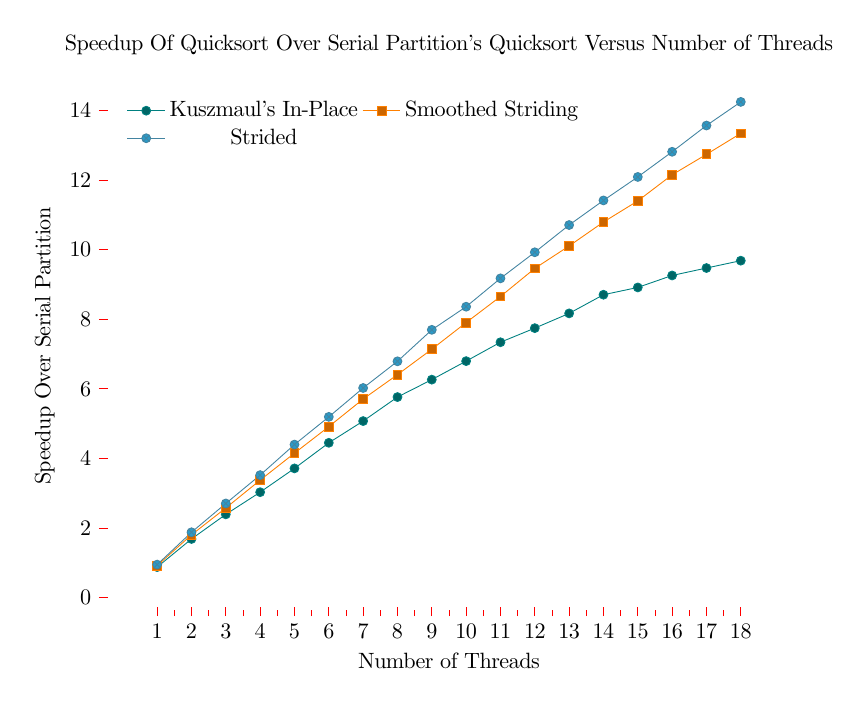
\begin{tikzpicture}[scale = .8]
\begin{axis}[
width = 5 in,
height = 4in,
title={Speedup Of Quicksort Over Serial Partition's Quicksort Versus Number of Threads},
xtick pos=left,
ytick pos=left,
legend style={draw=none},
axis line style = { draw = none },
legend pos= north west,
xtick = data,
xlabel={Number of Threads},
ylabel={Speedup Over Serial Partition},
ymax = 15,
legend columns = 2,
scatter/classes=%
{a={mark=o,draw=blue}}]
%% %% Low Space with log size 24
%% \addplot coordinates {( 1, 0.863202) ( 2, 1.63232) ( 3, 2.29705) ( 4, 2.96413) ( 5, 3.59298) ( 6, 4.1696) ( 7, 4.71085) ( 8, 5.2279) ( 9, 5.8474) ( 10, 6.4043) ( 11, 6.55736) ( 12, 7.21241) ( 13, 7.57064) ( 14, 7.99417) ( 15, 8.4679) ( 16, 8.93099) ( 17, 9.04881) ( 18, 9.60644) %% High-Span with log size 24
%% \addplot coordinates {( 1, 0.960106) ( 2, 1.88538) ( 3, 2.72075) ( 4, 3.47467) ( 5, 4.2576) ( 6, 5.08451) ( 7, 5.93339) ( 8, 6.47686) ( 9, 7.1822) ( 10, 7.57901) ( 11, 8.44704) ( 12, 8.64943) ( 13, 9.16979) ( 14, 9.04881) ( 15, 10.1464) ( 16, 9.61992) ( 17, 10.5199) ( 18, 9.38304) %% Cache Friendly with log size 24
%% \addplot coordinates {( 1, 0.900013) ( 2, 1.74752) ( 3, 2.46372) ( 4, 3.23233) ( 5, 3.90159) ( 6, 4.62508) ( 7, 5.46099) ( 8, 6.15157) ( 9, 6.85215) ( 10, 7.53736) ( 11, 8.11716) ( 12, 8.74872) ( 13, 9.70156) ( 14, 9.04881) ( 15, 11.0273) ( 16, 10.87) ( 17, 12.1829) ( 18, 12.2482) %% Strided with log size 24
%% \addplot coordinates {( 1, 0.95079) ( 2, 1.82955) ( 3, 2.63808) ( 4, 3.45716) ( 5, 4.20798) ( 6, 4.99199) ( 7, 5.78819) ( 8, 6.56364) ( 9, 7.37527) ( 10, 8.03162) ( 11, 8.89624) ( 12, 9.61992) ( 13, 9.7153) ( 14, 11.1167) ( 15, 10.9394) ( 16, 11.4891) ( 17, 13.1651) ( 18, 13.9695) };
%% %% Low Space with log size 26
%% \addplot coordinates {( 1, 0.861043) ( 2, 1.63325) ( 3, 2.3004) ( 4, 2.98343) ( 5, 3.63316) ( 6, 4.19898) ( 7, 4.82886) ( 8, 5.34581) ( 9, 5.89992) ( 10, 6.44372) ( 11, 6.94206) ( 12, 7.4672) ( 13, 7.60676) ( 14, 8.0564) ( 15, 8.64475) ( 16, 8.82709) ( 17, 8.76202) ( 18, 8.96831) %% High-Span with log size 26
%% \addplot coordinates {( 1, 0.955523) ( 2, 1.86586) ( 3, 2.6845) ( 4, 3.49224) ( 5, 4.27081) ( 6, 5.0929) ( 7, 5.83274) ( 8, 6.53586) ( 9, 7.29308) ( 10, 7.90003) ( 11, 8.63721) ( 12, 8.97915) ( 13, 9.7769) ( 14, 10.1893) ( 15, 10.5812) ( 16, 10.7887) ( 17, 10.7613) ( 18, 10.3418) %% Cache Friendly with log size 26
%% \addplot coordinates {( 1, 0.914609) ( 2, 1.73339) ( 3, 2.49178) ( 4, 3.22151) ( 5, 4.02384) ( 6, 4.70946) ( 7, 5.57239) ( 8, 6.13884) ( 9, 6.93881) ( 10, 7.59315) ( 11, 8.23047) ( 12, 8.91717) ( 13, 9.42939) ( 14, 10.1302) ( 15, 10.6801) ( 16, 10.8359) ( 17, 11.3883) ( 18, 11.3189) %% Strided with log size 26
%% \addplot coordinates {( 1, 0.946785) ( 2, 1.82922) ( 3, 2.64766) ( 4, 3.4262) ( 5, 4.2788) ( 6, 5.08245) ( 7, 5.95192) ( 8, 6.67986) ( 9, 7.44475) ( 10, 8.25563) ( 11, 8.94132) ( 12, 9.74164) ( 13, 10.4362) ( 14, 11.3621) ( 15, 11.4851) ( 16, 12.2071) ( 17, 12.6542) ( 18, 13.4993) };
%% %% Low Space with log size 28
%% \addplot coordinates {( 1, 0.862267) ( 2, 1.63941) ( 3, 2.34664) ( 4, 2.96157) ( 5, 3.64611) ( 6, 4.31258) ( 7, 4.88345) ( 8, 5.43042) ( 9, 5.87762) ( 10, 6.44029) ( 11, 7.00878) ( 12, 7.30452) ( 13, 7.83539) ( 14, 8.12956) ( 15, 8.50856) ( 16, 8.76302) ( 17, 8.98741) ( 18, 9.33821) %% High-Span with log size 28
%% \addplot coordinates {( 1, 0.939362) ( 2, 1.84744) ( 3, 2.6917) ( 4, 3.45716) ( 5, 4.29244) ( 6, 5.08279) ( 7, 5.79208) ( 8, 6.6353) ( 9, 7.2093) ( 10, 8.01682) ( 11, 8.74742) ( 12, 9.17326) ( 13, 9.7479) ( 14, 10.2979) ( 15, 11.0745) ( 16, 11.4344) ( 17, 11.4888) ( 18, 12.34) %% Cache Friendly with log size 28
%% \addplot coordinates {( 1, 0.908881) ( 2, 1.75263) ( 3, 2.51771) ( 4, 3.28228) ( 5, 4.01042) ( 6, 4.74982) ( 7, 5.54834) ( 8, 6.2393) ( 9, 6.98884) ( 10, 7.70125) ( 11, 8.41219) ( 12, 9.06778) ( 13, 9.67555) ( 14, 10.3505) ( 15, 11.0125) ( 16, 11.4744) ( 17, 12.1533) ( 18, 12.4095) %% Strided with log size 28
%% \addplot coordinates {( 1, 0.942529) ( 2, 1.82563) ( 3, 2.6044) ( 4, 3.46053) ( 5, 4.25683) ( 6, 5.12315) ( 7, 5.88602) ( 8, 6.70811) ( 9, 7.43113) ( 10, 8.17952) ( 11, 8.96974) ( 12, 9.68435) ( 13, 10.4214) ( 14, 10.9587) ( 15, 11.71) ( 16, 12.2949) ( 17, 12.9046) ( 18, 13.3107) };
%% Low Space with log size 30
\addplot coordinates {( 1, 0.87864) ( 2, 1.68661) ( 3, 2.39404) ( 4, 3.03172) ( 5, 3.71549) ( 6, 4.45118) ( 7, 5.07595) ( 8, 5.76618) ( 9, 6.26716) ( 10, 6.79929) ( 11, 7.34223) ( 12, 7.74736) ( 13, 8.17148) ( 14, 8.70784) ( 15, 8.91736) ( 16, 9.26139) ( 17, 9.47532) ( 18, 9.68665)}; %% High-Span with log size 30
%% \addplot coordinates {( 1, 0.96225) ( 2, 1.879) ( 3, 2.71741) ( 4, 3.56118) ( 5, 4.44821) ( 6, 5.29223) ( 7, 5.97895) ( 8, 6.76091) ( 9, 7.59373) ( 10, 8.37912) ( 11, 9.01587) ( 12, 9.58729) ( 13, 10.1906) ( 14, 10.881) ( 15, 11.4166) ( 16, 12.026) ( 17, 12.3279) ( 18, 12.6408)}; %% Cache Friendly with log size 30
\addplot coordinates {( 1, 0.921182) ( 2, 1.80562) ( 3, 2.57745) ( 4, 3.37831) ( 5, 4.15358) ( 6, 4.91613) ( 7, 5.7093) ( 8, 6.41041) ( 9, 7.14098) ( 10, 7.907) ( 11, 8.6573) ( 12, 9.46479) ( 13, 10.1098) ( 14, 10.7975) ( 15, 11.4046) ( 16, 12.1549) ( 17, 12.7427) ( 18, 13.346)}; %% Strided with log size 30
\addplot coordinates {( 1, 0.949951) ( 2, 1.87888) ( 3, 2.70758) ( 4, 3.52248) ( 5, 4.40049) ( 6, 5.19675) ( 7, 6.02708) ( 8, 6.79362) ( 9, 7.69896) ( 10, 8.36354) ( 11, 9.17828) ( 12, 9.92823) ( 13, 10.7114) ( 14, 11.4187) ( 15, 12.0935) ( 16, 12.8171) ( 17, 13.5719) ( 18, 14.2507) };
\legend{Kuszmaul's In-Place, Smoothed Striding, Strided}
\end{axis}
\end{tikzpicture}
}

%% Bandwith results without numactl:
%% \def \partitionbandwidthboundserialbaseline {3832}
%% \def \partitionbandwidthboundblocksize {64}
%% \def \partitionbandwidthboundnumtrials {5}
%% \def \partitionbandwidthboundinputsize {1073741824}
%% \def \partitionbandwidthboundtable {
%% \begin{tikzpicture}[scale = .8]
%% \begin{axis}[
%% width = 5 in,
%% height = 4in,
%% title={Speedup Versus Number of Threads},
%% xtick pos=left,
%% ytick pos=left,
%% legend style={draw=none},
%% axis line style = { draw = none },
%% legend pos= north west,
%% xtick = data,
%% xlabel={Number of Threads},
%% ylabel={Speedup Over Serial Partition},
%% ymax = 4,
%% legend columns = 2,
%% scatter/classes=%
%% {a={mark=o,draw=blue}}]
%% %% In-Place
%% \addplot coordinates {( 1, 0.504928) ( 2, 0.744917) ( 3, 1.27793) ( 4, 1.62967) ( 5, 1.91677) ( 6, 2.3244) ( 7, 2.47865) ( 8, 2.58186) ( 9, 2.68573) ( 10, 2.78448) ( 11, 2.7756) ( 12, 2.85077) ( 13, 2.86826) ( 14, 2.91407) ( 15, 2.90479) ( 16, 2.94769) ( 17, 2.95497) ( 18, 2.94588) };
%% %% Low-Space Bandwidth Bound
%% \addplot coordinates {(1, 1.05385)(2, 1.63936)(3, 1.81183)(4, 2.05614)(5, 2.39067)(6, 2.5237)(7, 2.40513)(8, 2.55015)(9, 2.58884)(10, 2.57444)(11, 2.69167)(12, 2.66946)(13, 2.64859)(14, 2.68175)(15, 2.66023)(16, 2.69318)(17, 2.68783)(18, 2.72913)};
%% %% high span
%% \addplot coordinates {( 1, 0.816814) ( 2, 1.47691) ( 3, 1.98529) ( 4, 2.63875) ( 5, 3.01305) ( 6, 3.40441) ( 7, 3.68887) ( 8, 3.97345) ( 9, 4.14181) ( 10, 4.27297) ( 11, 4.46724) ( 12, 4.45271) ( 13, 4.45271) ( 14, 4.62355) ( 15, 4.60024) ( 16, 4.70184) ( 17, 4.55431) ( 18, 4.71225) };
%% %% High-Span Bandwidth Bound
%% \addplot coordinates {(1, 2.03744)(2, 3.14521)(3, 3.47353)(4, 3.91661)(5, 4.536)(6, 4.70395)(7, 4.47075)(8, 4.76355)(9, 4.86065)(10, 4.68934)(11, 4.86418)(12, 4.98468)(13, 4.9239)(14, 4.99117)(15, 4.94174)(16, 4.98761)(17, 4.96382)(18, 5.00564)%% cache friendly
%% \addplot coordinates {( 1, 0.621291) ( 2, 1.06581) ( 3, 1.76541) ( 4, 2.28204) ( 5, 2.8838) ( 6, 3.49253) ( 7, 4.04561) ( 8, 4.56843) ( 9, 4.97921) ( 10, 5.6089) ( 11, 5.8791) ( 12, 6.26963) ( 13, 6.8331) ( 14, 6.87971) ( 15, 7.15459) ( 16, 7.38343) ( 17, 8.25151) ( 18, 8.35587) };
%% %% Cache-Friendly Bandwidth Bound
%% \addplot coordinates {(1, 4.06363)(2, 6.29023)(3, 6.9299)(4, 7.88794)(5, 9.08502)(6, 9.329)(7, 9.45987)(8, 9.53406)(9, 9.91163)(10, 9.90729)(11, 9.70433)(12, 10.1146)(13, 9.9126)(14, 9.85886)(15, 9.86993)(16, 10.0183)(17, 10.0765)(18, 9.99261)};
%% \legend{Low-Space, Low-Space Bandwidth Constraint, Two-Layer, Two-Layer Bandwidth Constraint}
%% \end{axis}
%% \end{tikzpicture}
%% }

\def \serialnumtrials {5}
\def \serialblocksize {64}
\def \serialtable {
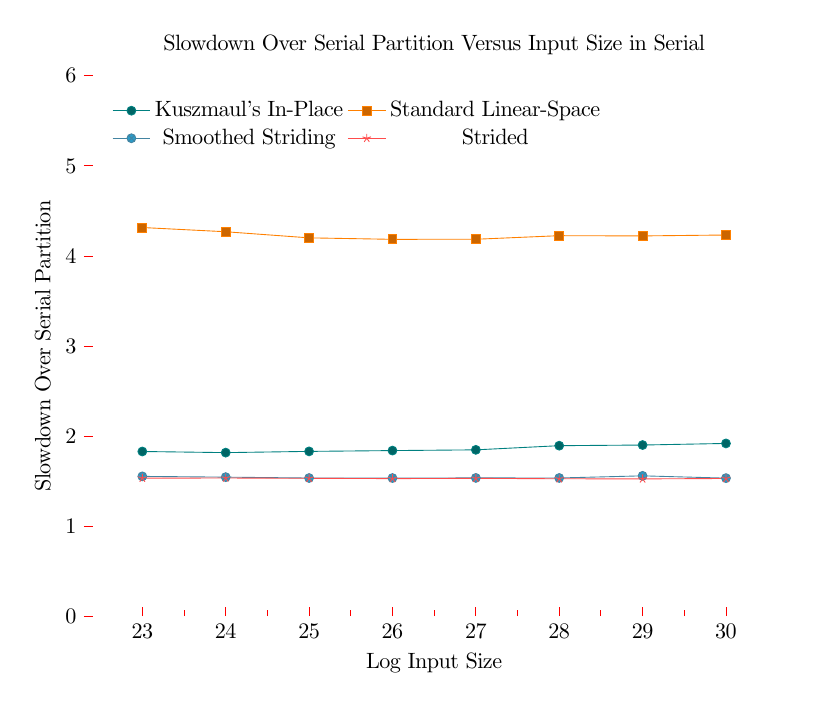
\begin{tikzpicture}[scale = .8]
\begin{axis}[
width = 5 in,
height = 4in,
title={Slowdown Over Serial Partition Versus Input Size in Serial},
xtick pos=left,
ytick pos=left,
ymax = 6,
ymin = 0,
legend style={draw=none},
axis line style = { draw = none },
legend pos= north west,
xtick = data,
xlabel={Log Input Size},
ylabel={Slowdown Over Serial Partition},
legend columns = 2,
scatter/classes=%
{a={mark=o,draw=blue}}]
%% Serial Baseline
%% baselines in ms: \addplot coordinates {( 23, 30.4 ) ( 24, 61 ) ( 25, 122.4 ) ( 26, 244.8 ) ( 27, 489.6 ) ( 28, 979.6 ) ( 29, 1963.4 ) ( 30, 3922.6 ) };
%% In-Place
\addplot coordinates {( 23, 1.82895) ( 24, 1.81639) ( 25, 1.83007) ( 26, 1.83905) ( 27, 1.84722) ( 28, 1.89343) ( 29, 1.90068) ( 30, 1.91837) };
%% In-Place Prefix-Sum
% \addplot coordinates {( 23, 2.75658) ( 24, 2.71803) ( 25, 2.68137) ( 26, 2.67157) ( 27, 2.67443) ( 28, 2.70131) ( 29, 2.70551) ( 30, 2.71713) };
%% Out-of-Place
\addplot coordinates {( 23, 4.31579) ( 24, 4.26885) ( 25, 4.20098) ( 26, 4.18464) ( 27, 4.18546) ( 28, 4.22519) ( 29, 4.22257) ( 30, 4.23265) };
%% %% High-Span
%% \addplot coordinates {( 23, 1.23684) ( 24, 1.23934) ( 25, 1.24346) ( 26, 1.24428) ( 27, 1.24632) ( 28, 1.24602) ( 29, 1.24417) ( 30, 1.2456) };
%% Cache-Friendly
\addplot coordinates {( 23, 1.55263) ( 24, 1.54426) ( 25, 1.53431) ( 26, 1.53431) ( 27, 1.53554) ( 28, 1.53491) ( 29, 1.55852) ( 30, 1.53317) };
%% Strided
\addplot coordinates {( 23, 1.53289) ( 24, 1.53443) ( 25, 1.53105) ( 26, 1.52778) ( 27, 1.53064) ( 28, 1.52613) ( 29, 1.5246) ( 30, 1.52919) };
\legend{Kuszmaul's In-Place, Standard Linear-Space, Smoothed Striding, Strided} % Low-Space, Med-Space, High-Space, Smoothed Striding, Strided
\end{axis}
\end{tikzpicture}
}
%% \def \serialnumtrials {5}
%% \def \serialblocksize {64}
%% \def \serialtable {
%% \begin{tikzpicture}[scale = .8]
%% \begin{axis}[
%% width = 5 in,
%% height = 4in,
%% title={Slowdown Versus Input Size in Serial},
%% xtick pos=left,
%% ytick pos=left,
%% ymax = 5,
%% ymin = 0,
%% legend style={draw=none},
%% axis line style = { draw = none },
%% legend pos= north west,
%% xtick = data,
%% xlabel={Log Input Size},
%% ylabel={Slowdown Over Serial Partition},
%% legend columns = 2,
%% scatter/classes=%
%% {a={mark=o,draw=blue}}]
%% %% Serial Baseline
%% %% baselines in ms: \addplot coordinates {( 23, 30.4 ) ( 24, 61 ) ( 25, 122.4 ) ( 26, 244.8 ) ( 27, 489.6 ) ( 28, 979.6 ) ( 29, 1963.4 ) ( 30, 3922.6 ) };
%% %% In-Place
%% \addplot coordinates {( 23, 1.82895) ( 24, 1.81639) ( 25, 1.83007) ( 26, 1.83905) ( 27, 1.84722) ( 28, 1.89343) ( 29, 1.90068) ( 30, 1.91837) };
%% %% In-Place Prefix-Sum
%% \addplot coordinates {( 23, 2.75658) ( 24, 2.71803) ( 25, 2.68137) ( 26, 2.67157) ( 27, 2.67443) ( 28, 2.70131) ( 29, 2.70551) ( 30, 2.71713) };
%% %% Out-of-Place
%% \addplot coordinates {( 23, 4.31579) ( 24, 4.26885) ( 25, 4.20098) ( 26, 4.18464) ( 27, 4.18546) ( 28, 4.22519) ( 29, 4.22257) ( 30, 4.23265) };
%% %% High-Span
%% \addplot coordinates {( 23, 1.23684) ( 24, 1.23934) ( 25, 1.24346) ( 26, 1.24428) ( 27, 1.24632) ( 28, 1.24602) ( 29, 1.24417) ( 30, 1.2456) };
%% %% Cache-Friendly
%% \addplot coordinates {( 23, 1.55263) ( 24, 1.54426) ( 25, 1.53431) ( 26, 1.53431) ( 27, 1.53554) ( 28, 1.53491) ( 29, 1.55852) ( 30, 1.53317) };
%% %% Strided
%% \addplot coordinates {( 23, 1.53289) ( 24, 1.53443) ( 25, 1.53105) ( 26, 1.52778) ( 27, 1.53064) ( 28, 1.52613) ( 29, 1.5246) ( 30, 1.52919) };
%% \legend{Low-Space, Med-Space, High-Space, Two-Layer, Cache-Friendly, Strided}
%% \end{axis}
%% \end{tikzpicture}
%% }
%% \def \serialnumtrials {1}
%% \def \serialblocksize {64}
%% \def \serialtable {
%% \begin{tikzpicture}[scale = .8]
%% \begin{axis}[
%% title={Slowdown Versus Input Size in Serial},
%% width = 5in, %%!!!!
%% height = 4in,
%% xtick pos=left,
%% ytick pos=left,
%% ymax = 5, %% !!!
%% ymin = 0,
%% legend style={draw=none},
%% axis line style = { draw = none },
%% legend pos= north west,
%% xtick = data,
%% xlabel={Log Input Size},
%% ylabel={Slowdown Over Serial Partition},
%% legend columns = 2,
%% scatter/classes=%
%% {a={mark=o,draw=blue}}]
%% %% Serial Baseline%% baselines in ms: \addplot coordinates {( 23, 30.4 ) ( 24, 60.8 ) ( 25, 121.4 ) ( 26, 243.8 ) ( 27, 487.4 ) ( 28, 975.8 ) ( 29, 1952.2 ) ( 30, 3902 ) };
%% %% In-Place
%% \addplot coordinates {( 23, 1.79605) ( 24, 1.82237) ( 25, 1.84185) ( 26, 1.84249) ( 27, 1.87033) ( 28, 1.90838) ( 29, 1.90687) ( 30, 1.91579) };
%% %% In-Place Prefix-Sum
%% \addplot coordinates {( 23, 2.58553) ( 24, 2.57237) ( 25, 2.57661) ( 26, 2.56932) ( 27, 2.56422) ( 28, 2.59459) ( 29, 2.60834) ( 30, 2.61107) };
%% %% Out-of-Place
%% \addplot coordinates {( 23, 3.98684) ( 24, 3.96711) ( 25, 3.96705) ( 26, 3.96308) ( 27, 3.98195) ( 28, 4.01537) ( 29, 4.03401) ( 30, 4.06079) };
%% %% High-Span
%% \addplot coordinates {( 23, 1.21053) ( 24, 1.23355) ( 25, 1.23558) ( 26, 1.23298) ( 27, 1.23677) ( 28, 1.24124) ( 29, 1.24096) ( 30, 1.23931) };
%% \legend{Low-Space, Med-Space, High-Space, Two-Layer} %% Two-layer instead of high-span everywhere
%% \end{axis}
%% \end{tikzpicture}
%% }
%% %% Speedup on 18 threads in table of size 268435456
%% \def \serialsortspeedup {0.780189}


\newcommand{\dec}{\operatorname{dec}}
\newcommand{\poly}{\operatorname{poly}}
\newcommand{\polylog}{\operatorname{polylog}}
\newcommand{\github}{\url{github.com/awestover/Parallel-Partition}}
\newcommand{\defn}[1]       {{\textit{\textbf{\boldmath #1}}}}
\renewcommand{\paragraph}[1]{\vspace{0.09in}\noindent{\bf \boldmath #1.}} 
\usepackage{amsmath}
\def\E{\operatorname{\mathbb{E}}}
\usepackage{amssymb}
\usepackage{amsthm}
\usepackage{todonotes}

\newtheorem{thm}{Theorem}[section]
\newtheorem{lem}[thm]{Lemma}
\newtheorem{prop}[thm]{Proposition}
\newtheorem{clm}[thm]{Claim}
\newtheorem{cor}[thm]{Corollary}
\newtheorem{conj}[thm]{Conjecture}
\theoremstyle{remark}
\newtheorem{rem}[thm]{Remark}
\newtheorem{ex}[thm]{Example}

\newtheorem{theorem}{Theorem}[section]
\newtheorem{definition}[thm]{Definition}
\newtheorem{lemma}[thm]{Lemma}
\newtheorem{proposition}[thm]{Proposition}
\newtheorem{claim}[thm]{Claim}
\newtheorem{corollary}[thm]{Corollary}
\newtheorem{conjecture}[thm]{Conjecture}
\theoremstyle{remark}
\newtheorem{remark}[thm]{Remark}
\newtheorem{example}[thm]{Example}
\newtheorem{observation}[thm]{Observation}

\usepackage{hyperref}



\begin{document}
\title[]{In-Place Parallel-Partition Algorithms using Exclusive-Read-and-Write Memory}
\subtitle{}

\author{William Kuszmaul}
\authornote{Supported by a Hertz Fellowship and a NSF GRFP Fellowship}
\affiliation{%
  \institution{Massachusetts Institute of Technology}
}
\email{kuszmaul@mit.edu}


\author{Alek Westover}
\authornote{Supported by MIT PRIMES.}
\email{alek.westover@gmail.com}


% The default list of authors is too long for headers.
\renewcommand{\shortauthors}{William Kuszmaul}


\begin{abstract}
We present an in-place algorithm for the parallel partition problem that has work $O(n)$ and span $O(\log n \cdot \log \log n)$. The algorithm uses only exclusive read/write shared variables, and can be implemented using parallel-for-loops without any additional concurrency considerations (i.e., the algorithm is EREW). As an immediate consequence, we also get an in-place quicksort algorithm with work $O(n \log n)$ and span $O(\log^2 n \log \log n)$.

Using our algorithmic techniques, we implement an (almost) in-place parallel partition. In addition to achieving much better memory utilization, the algorithm leverages its improved cache behavior to achieve a speedup over its out-of-place counterpart. Both algorithms remain bottlenecked by memory bandwidth, however, due to the fact that they require multiple passes over the input array.

Our second contribution is an in-place EREW algorithm with polylogarithmic span and provably optimal cache behavior, up to small-order factors.  The resulting algorithm achieves near-ideal scaling in practice by avoiding the memory-bandwidth bottleneck. The algorithm's performance is comparable to that the Blocked Strided Algorithm of Francis, Pannan, Frias, and Petit, which is the previous state-of-the art for parallel EREW sorting algorithms, but which lacks theoretical guarantees on its span and cache behavior.
\end{abstract}

%
% The code below should be generated by the tool at
% http://dl.acm.org/ccs.cfm
% Please copy and paste the code instead of the example below.
%
%% \begin{CCSXML}
%% <ccs2012>
%% <concept>
%% <concept_id>10003752.10003809.10010170.10010171</concept_id>
%% <concept_desc>Theory of computation~Shared memory algorithms</concept_desc>
%% <concept_significance>500</concept_significance>
%% </concept>
%% </ccs2012>
%% \end{CCSXML}

%% \ccsdesc[500]{Theory of computation~Shared memory algorithms}

%% \keywords{Parallel Partition, EREW PRAM, in-place algorithms}


\maketitle





 

\section{Introduction}

A \defn{parallel partition} operation rearranges the elements in an
array so that the elements satisfying a particular \defn{pivot
  property} appear first. In addition to playing a central role in
parallel quicksort, the parallel partition operation is used as a
primitive throughout parallel algorithms.\footnote{In several
  well-known textbooks and surveys on parallel algorithms
  \cite{AcarBl16,Blelloch96}, for example, parallel partitions are
  implicitly used extensively to perform what are referred to as
  \emph{filter} operations.}

A parallel algorithm can be measured by its \defn{work}, the time
needed to execute in serial, and its \defn{span}, the time to execute
on infinitely many processors. There is a well-known algorithm for
parallel partition on arrays of size $n$ with work $O(n)$ and span
$O(\log n)$ \cite{Blelloch96,AcarBl16}. Moreover, the algorithm uses
only exclusive read/write shared memory variables (i.e., it is an
\defn{EREW} algorithm). This eliminates the need for concurrency
mechanisms such as locks and atomic variables, and ensures good
behavior even if the time to access a location is a function of the
number of threads trying to access it (or its cache line)
concurrently. EREW algorithms also have the advantage that their
behavior is internally deterministic, meaning that
the behavior of the algorithm will not differ from run to run, which
makes test coverage, debugging, and reasoning about performance
substantially easier \cite{BlellochFi12}.

The parallel-partition algorithm suffers from using a large amount of
auxiliary memory, however. Whereas the serial algorithm is typically
implemented in place, the parallel algorithm relies on the use of two
auxiliary arrays of size $n$. To the best of our knowledge, the only
known linear-work and $\operatorname{polylog}(n)$-span algorithms for
parallel partition that are in-place require the use of atomic
operations (e.g, fetch-and-add)
\cite{HeidelbergerNo90,AxtmannWi17,TsigasZh03}.

An algorithm's memory efficiency can be critical on large inputs. The
memory consumption of an algorithm determines the largest problem size
that can be executed in memory. Many external memory algorithms (i.e.,
algorithms for problems too large to fit in memory) perform large
subproblems in memory; the size of these subproblems is again
bottlenecked by the algorithm's memory-overhead \cite{Vitter08}. In
multi-user systems, processes with larger memory-footprints can hog
the cache and the memory bandwidth, slowing down other processes.

For sorting algorithms, in particular, special attention to memory
efficiency is often given. This is because (a) a user calling the sort
function may already be using almost all of the memory in the system;
and (b) sorting algorithms, and especially parallel sorting
algorithms, are often bottlenecked by memory bandwidth. The latter
property, in particular, means that any parallel sorting algorithm
that wishes to achieve state-of-the art performance on a large
multi-processor machine must be (at least close to) in place.

Currently the only practical in-place parallel sorting algorithms
either rely heavily on atomic operations or other concurrency
mechanisms \cite{HeidelbergerNo90, AxtmannWi17, TsigasZh03}, or eschew
theoretical guarantees \cite{FrancisPa92}. Parallel merge sort
\cite{Hagerup89} was made in-place by Katajainen \cite{Katajainen93},
but has proven too sophisticated for practical applications. Bitonic
sort \cite{BlellochLe98} is naturally in-place, and can be practical
in certain applications on super computers, but suffers in general
from requiring work $\Theta(n \log^2 n)$ rather than $O(n \log
n)$. Parallel quicksort, on the other hand, despite the many efforts
to optimize it \cite{HeidelbergerNo90, AxtmannWi17, TsigasZh03,
  FrancisPa92, Frias08}, has eluded any in-place EREW (or CREW)
algorithms due to its reliance on parallel partition.\footnote{In aCRCW
  \defn{CREW} algorithm, reads may be concurrent, but writes may
  not. CREW stands for \emph{concurrent-read exclusive-write}.}

\paragraph{Results}
We show that parallel partition can be implemented in place, and
without the use of concurrency mechanisms. All of the algorithms
considered in this paper use only exclusive read/write shared
variables, and can be implemented using parallel-for-loops without any
additional concurrency considerations. 

Our first result is a set of techniques that allows us to adapt the
standard parallel partition algorithm to be fully in place. The new
algorithm has work $O(n)$ and span $O(\log n \cdot \log \log
n)$. As an immediate consequence, we also get a
simple in-place quicksort algorithm with work $O(n \log n)$ and span
$O(\log^2 n \log \log n)$.

Using our algorithmic techniques, we implement and optimize a
space-efficient parallel partition. Because the in-place algorithm
eliminates the use of large auxiliary arrays, the algorithm is able to
achieve a significant reduction in cache misses over its out-of-place
counterpart, resulting in performance improvements both in serial and
in parallel over the standard parallel partition algorithm.

The in-place algorithm remains bottlenecked by memory bandwidth,
however, due to the fact that multiple passes over the input array are
required. The memory-bandwidth bottleneck has led past researchers
\cite{FrancisPa92, Frias08} to introduce the so-called \defn{Strided
  Algorithm}, which has near optimal cache behavior in practice, but
which exhibits theoretical guarantees only on certain random input
arrays.

Our second main result is an algorithm that we call the \defn{Smoothed
  Striding Algorithm}. By randomly perturbing the internal structure
of the Strided Algorithm, and adding a recursion step that was
previously not possible, we arrive at a new algorithm with provably
good span and cache behavior. The Smoothed Striding Algorithm is
in-place, has polylogarithmic span, and exhibits provably optimal
cache behavior up to small-order factors. In practice, the Smoothed
Striding Algorithm performs within 15\% of the Strided Algorithm on a
large number of threads.



\section{Preliminaries}\label{secprelim}

We begin by describing the the parallelism and memory model used in
the paper, and by presenting background on parallel partition.

\paragraph{Workflow Model} We consider a simple language-based model of parallelism in which algorithms achieve parallelism through the use of \defn{parallel-for-loops} (see, e.g.,
\cite{Blelloch96,AcarBl16,CLRS}); function calls within the inner loop
then allow for more complicated parallel structures (e.g., recursion). Our algorithms can also be implemented in the less restrictive PRAM model \cite{Blelloch96, AcarBl16}.

Formally, a parallel-for-loop is given a range $R \in \mathbb{N}$, a
constant number of arguments $\arg_1, \arg_2, \ldots, \arg_c$, and a
body of code. For each $i \in \{1, \ldots, R\}$, the loop launches a
thread that is given loop-counter $i$ and local copies of the
arguments $\arg_1, \arg_2, \ldots, \arg_c$. The threads are then taken up by processors and the iterations of the loop are performed in parallel. Only after every iteration of the loop is complete can control flow continue past the loop.

A parallel algorithm may be run on an arbitrary number $p$ of
processors. The algorithm itself is oblivious to $p$, however, leaving
the assignment of threads to processors up to a scheduler.

The \defn{work} $T_1$ of an algorithm is the time that the algorithm
would require to execute on a single processor. The \defn{span}
$T_\infty$ of an algorithm is the time to execute on infinitely many
processors. The scheduler is assumed to contribute no overhead to the
span. In particular, if each iteration of a
parallel-for-loop has span $s$, then the full parallel loop has span
$s + O(1)$ \cite{Blelloch96,AcarBl16}.

The work $T_1$ and span $T_\infty$ can be used to quantify the time $T_p$
that an algorithm requires to execute on $p$ processors using a greedy
online scheduler. If the scheduler is assumed to contribute no
overhead, then Brent's Theorem \cite{Brent74} states that for any
$p$,
$$T_1 / p \le T_p \le T_1 / p + T_\infty.$$

The work-stealing algorithms used in the Cilk extension of C/C++ realize
the guarantee offered by Brent's Theorem within a constant factor
\cite{BlumofeJo96,BlumofeLe99}, with the added caveat that parallel-for-loops typically induce an additional additive overhead of $O(\log
R)$. 

\paragraph{Memory Model} Memory is \defn{exclusive-read} and \defn{exclusive-write}. That is, no two threads are ever permitted to attempt to read or write to the same variable concurrently. 
The exclusive-read exclusive-write memory model is sometime referred
to as the \defn{EREW model} (see, e.g., \cite{Hagerup89}).

Note that threads are not in lockstep (i.e., they may progress at arbitrary different speeds), and thus the EREW model requires algorithms to be data-race free in order to avoid the possibility of non-exclusive data accesses.

In an \defn{in-place} algorithm, each thread is given $O(\polylog n)$
memory upon creation that is deallocated when the thread dies. This
memory can be shared with the thread's children. However, the depth of
the parent-child tree is not permitted to exceed $O(\polylog n)$.

Whereas the EREW memory model prohibits concurrent accesses to memory, on the other side of the spectrum are CRCW (concurrent-read-concurrent-write) models, which allow for both reads and writes to be performed concurrently (and in some variants even allow for atomic operations) \cite{Blelloch96,AcarBl16,MatiasVi95}. One approach to designing efficient EREW algorithms is to simulate efficient CRCW algorithms in the EREW model \cite{MatiasVi95}. The known simulation techniques require substantial space overhead, however, preventing the design of in-place algorithms \cite{MatiasVi95}.\footnote{The known simulation techniques also increase the total work in the original algorithm, although this can be acceptable if only a small number of atomic operations need to be simulated.}

%% HERE: Is where we can talk about the more powerful alternative to EREW, and there relationship, and why we can't just simulate CRCW (or, more importantly, ERCW). Make it clear that the Exclusive Read part is not actually very important -- it's the exclusive write part that's hard.

%% \footnote{The
  %% algorithm in this paper satisfies a slightly stronger property that
  %% the total memory being used is never more than $O(\log n) \cdot p$,
  %% where $p$ is an upper-bound on the number of worker threads.}

\paragraph{The Parallel Partition Problem}
The parallel partition problem takes an input array $A$ of size $n$,
and a \defn{decider function} $\dec$ that determines for each element
$A[i] \in A$ whether or not $A[i]$ is a \defn{predecessor} or a
\defn{successor}. That is, $\dec(A[i]) = 1$ if $A[i]$ is a
predecessor, and $\dec(A[i]) = 0$ if $A[i]$ is a successor. The
behavior of the parallel partition is to reorder the elements in the
array $A$ so that the predecessors appear before the successors.


\paragraph{The (Standard) Linear-Space Parallel Partition} The linear-space implementation of parallel partition consists of two phases \cite{Blelloch96,AcarBl16}:

\noindent\emph{The Parallel-Prefix Phase: }In this phase, the algorithm
constructs an array $B$ whose $i$-th element $B[i] = \sum_{j = 1}^i
\dec(A[i])$ is the number of predecessors in the first $i$ elements of
$A$. The transformation from $A$ to $B$ is called a \defn{parallel
  prefix sum} and can be performed with $O(n)$ work and $O(\log n)$
span using a simple recursive algorithm: (1) First construct an array
$A'$ of size $n / 2$ with $A'[i] = A[2i - 1] + A[2i]$; (2)
Recursively construct a parallel prefix sum $B'$ of $A'$; (3) Build
$B$ by setting each $B[i] = B'[\lfloor i / 2 \rfloor] + A[i]$ for odd
$i$ and $B[i] = A'[i / 2]$ for even $i$. 

\noindent\emph{The Reordering Phase: }In this phase, the algorithm
constructs an output-array $C$ by placing each predecessor $A[i] \in A$
in position $B[i]$ of $C$. If there are $t$ predecessors in $A$, then
the first $t$ elements of $C$ will now contain those $t$ predecessors
in the same order that they appear in $A$. The algorithm then places
each successor $A[i] \in A$ in position $t + i - B[i]$. Since $i - B[i]$
is the number of successors in the first $i$ elements of $A$, this
places the successors in $C$ in the same order that they appear in
$A$. Finally, the algorithm copies $C$ into $A$, completing the
parallel partition.

Both phases can be implemented with $O(n)$ work and $O(\log n)$
span. Like its serial out-of-place counterpart, the algorithm is
stable but not in place. The algorithm uses two auxiliary arrays of
size $n$. Kiu, Knowles, and Davis \cite{LiuKn05} were able to reduce
the extra space consumption to $n + p$ under the assumption that the
number of processors $p$ is hard-coded; their algorithm breaks the
array $A$ into $p$ parts and assigns one part to each thread. Reducing
the space below $o(n)$ has remained open until now, even when the
number of threads is fixed.

\section{An In-Place Algorithm with Span $O(\log n \log \log n)$}\label{secalg}

In this section, we present an in-place algorithm for parallel
partition with span $O(\log n \log \log n)$. Each thread in the
algorithm requires memory at most $O(\log n)$.

We assume without loss of generality that the total number of
successors in $A$ exceeds the number of predecessors, since otherwise
their roles can simply be swapped in the algorithm. Further, we assume
for simplicity that the elements of $A$ are distinct; this assumption
is removed at the end of the section.


\paragraph{Algorithm Outline}
We begin by presenting an overview of the key algorithmic ideas needed
to construct an in-place algorithm.

Consider how to remove the auxiliary array $C$ from the Reordering
Phase. If one attempts to simply swap in parallel each predecessor
$A[i]$ with the element in position $j = B[i]$ of $A$, then the swaps
will almost certainly conflict. Indeed, $A[j]$ may also be a
predecessor that needs to be swapped with $A[B[j]]$. Continuing like
this, there may be an arbitrarily long list of dependencies on the
swaps.

To combat this, we begin the algorithm with a Preprocessing Phase in
which $A$ is rearranged so that every prefix is
\defn{successor-heavy}, meaning that for all $t$, the first $t$
elements contain at least $\frac{t}{4}$ successors. Then we compute
the prefix-sum array $B$, and begin the Reordering Phase. Using the
fact that the prefixes of $A$ are successor-heavy, the reordering can
now be performed in place as follows: (1) We begin by recursively
reordering the prefix $P$ of $A$ consisting of the first $4/5 \cdot n$
elements, so that the predecessors appear before the successors; (2)
Then we simply swap each predecessor $A[i]$ in the final $1/5 \cdot n$
elements with the corresponding element $B[A[i]]$. The fact that the
prefix $P$ is successor-heavy ensures that the final $\frac{1}{5}
\cdot n$ elements of the reordered $P$ will consist of
successors. This implies that for each of the swaps between
predecessors $A[i]$ in the final $1/5 \cdots n$ elements and earlier
positions $B[A[i]]$, the latter element will be a successor. In other
words, the swaps are now conflict free.

Next consider how to remove the array $B$ from the Parallel-Prefix
Phase. At face value, this would seem quite difficult since the
reordering phase relies heavily on $B$. Our solution is to
\emph{implicitly} store the value of every $O(\log n)$-th element of
$B$ in the ordering of the elements of $A$. That is, we break $A$ into
blocks of size $O(\log n)$, and use the order of the elements in each
block to encode an entry of $B$. (If the elements are not all
  distinct, then a slightly more sophisticated encoding is necessary.)
Moreover, we modify the algorithm for building $B$ to only construct
every $O(\log n)$-th element. The new parallel-prefix sum performs
$O(n / \log n)$ arithmetic operations on values that are implicitly
encoded in blocks; since each such operation requires $O(\log n)$
work, the total work remains linear.

In the remainder of the section, we present the algorithm in detail.
It proceeds in three phases.

\paragraph{A Preprocessing Phase}
The goal of the Preprocessing phase is to make every prefix of $A$
successor-heavy. To perform the Preprocessing phase on $A$, we begin
with a parallel-for-loop: For each $i = 1, \ldots, \lfloor n /
2\rfloor$, if $A[i]$ is a predecessor and $A[n - i + 1]$ is a
successor, then we swap their positions in $A$. To complete the
Preprocessing phase on $A$, we then recursively perform a
Preprocessing phase on $A[1], \ldots, A[\lceil n / 2 \rceil]$.

\begin{lemma}
 The Preprocessing Phase has work $O(n)$ and span $O(\log n)$. At the
 end of the Preprocessing Phase, every prefix of $A$ is
 successor-heavy.
  \label{lem:preprocessingphase}
\end{lemma}
\begin{proof}
Recall that for each $t \in 1, \ldots, n$, we call the $t$-prefix
$A[1], \ldots, A[t]$ of $A$ successor-heavy if it contains at least
$\frac{t}{4}$ successors.

The first parallel-for-loop ensures that at least half the successors
in $A$ reside in the first $\lceil n / 2 \rceil$ positions, since for
$i = 1, \ldots, \lfloor n / 2 \rfloor$, $A[n - i + 1]$ will only be a
successor if $A[i]$ is also a successor. Because at least half the
elements in $A$ are successors, it follows that the first $\lceil n /
2 \rceil$ positions contain at least $\lceil n / 4\rceil$ successors,
making every $t$-prefix with $t \ge \lceil n / 2 \rceil$
successor-heavy.

After the parallel-for-loop, the first $\lceil n / 2 \rceil$ positions
of $A$ contain at least as many successors as predecessors (since
$\lceil n / 4 \rceil \ge \frac{\lceil n / 2 \rceil}{2}$). Thus we can
recursively apply the argument above in order to conclude that the
recursion on $A[1], \ldots, A[\lceil n / 2 \rceil]$ makes every
$t$-prefix with $t \le \lceil n / 2 \rceil$ successor-heavy. It
follows that, after the recursion, every $t$-prefix of $A$ is
successor-heavy.

Each recursive level has constant span and performs work proportional
to the size of the subarray being considered. The Preprocessing phase
therefore has total work $O(n)$ and span $O(\log n)$.
\end{proof}


%% Recall that for each $t \in 1, \ldots, n$, we call the $t$-prefix
%% $A[1], \ldots, A[t]$ of $A$ successor-heavy if it contains at least
%% $\frac{t}{4}$ successors. The goal of the preprocessing phase is to
%% rearrange $A$ so that every prefix is successor heavy.

%% We begin with a parallel-for-loop: For each $i = 1, \ldots, \lfloor n
%% / 2\rfloor$, if $A[i]$ is a predecessor and $A[n - i + 1]$ is a
%% successor, then we swap their positions in $A$.

%% This ensures that at least half the successors in $A$ reside in the
%% first $\lceil n / 2 \rceil$ positions. Thus the first $\lceil n / 2
%% \rceil$ positions contain at least $\lceil n / 4\rceil$ successors,
%% making every $t$-prefix with $t \ge \lceil n / 2 \rceil$
%% successor-heavy.

%% Since $\lceil n / 4 \rceil \ge \frac{\lceil n / 2 \rceil}{2}$, the
%% first $\lceil n / 2 \rceil$ positions of $A$ now contain at least as
%% many successors as predecessors. Thus we can recursively repeat the
%% same process on the subarray $A[1], \ldots, A[\lceil n / 2 \rceil]$
%% in order to make each of its prefixes successor-heavy.

%% Each recursive step has constant span and performs work proportional
%% to the size of the subarray being considered. The preprocessing phase
%% therefore has total work $O(n)$ and span $O(\log n)$.

\paragraph{An Implicit Parallel Prefix Sum}
Pick a \defn{block-size} $b \in \Theta(\log n)$ satisfying $b \ge 2
\lceil \log (n + 1) \rceil$. Consider $A$ as a series of $\lfloor n /
b \rfloor$ blocks of size $b$, with the final block of size between
$b$ and $2b - 1$. Denote the blocks by $X_1, \ldots, X_{\lfloor n / b
  \rfloor}$.

Within each block $X_i$, we can implicitly store a value in the range
$0, \ldots, n$ through the ordering of the elements:
\begin{lemma}
Given an array $X$ of $2 \lceil \log (n + 1) \rceil$ distinct
elements, and a value $v \in \{0, \ldots, n\}$, one can rearrange the
elements of $X$ to encode the bits of $v$ using work $O(\log n)$ and
span $O(\log \log n)$; and one can then later decode $v$ from $X$
using work $O(\log n)$ and span $O(\log \log n)$.
\label{lem:bitstore}
\end{lemma}
\begin{proof}
Observe that $X$ can be broken into (at least) $\lceil \log (n + 1)
\rceil$ disjoint pairs of adjacent elements $(x_1, x_2), (x_3, x_4),
\ldots$, and by rearranging the order in which a given pair $(x_j,
x_{j + 1})$ occurs, the lexicographic comparison of whether $x_j <
x_{j + 1}$ can be used to encode one bit of information. Values $v \in
[0,n]$ can therefore be read and written to $X$ with work $O(b) =
O(\log n)$ and span $O(\log b) = O(\log \log n)$ using a simple
divide-and-conquer recursive approach to encode and decode the bits of
$v$.
\end{proof}

To perform the Parallel Prefix Sum phase, our algorithm beings by
performing a parallel-for loop through the blocks, and storing in each
block $X_i$ a value $v_i$ equal to the number of predecessors in the
block. (This can be done in place with work $O(n)$ and span $O(\log
\log n)$ by Lemma \ref{lem:bitstore}.)

The algorithm then performs an in-place parallel-prefix operation on
the values $v_1, \ldots, v_{\lfloor n / b \rfloor}$ stored in the
blocks. This is done by first resetting each even-indexed value
$v_{2i}$ to $v_{2i} + v_{2i - 1}$; then recursively performing a
parallel-prefix sum on the even-indexed values; and then replacing
each odd-indexed $v_{2i + 1}$ with $v_{2i + 1} + v_{2i}$, where $v_0$
is defined to be zero.

Lemma \ref{lem:parallelprefix} analyzes the phase:
\begin{lemma}
The Parallel Prefix Sum phase uses work $O(n)$ and span $O(\log n \log
\log n)$. At the end of the phase, each $X_i$ encodes a value $v_i$
counting the number of predecessors in the prefix $X_1 \circ X_2 \circ
\cdots \circ X_i$; and each prefix $X_1 \circ X_2 \circ \cdots \circ
X_i$ is successor-heavy.
\label{lem:parallelprefix}
\end{lemma}
\begin{proof}
If the $v_i$'s could be read and written in constant time, then the
prefix sum would take work $O(n / \log n)$ and span $O(\log n)$, since
there are $O(n / \log n)$ $v_i$'s. Because each $v_i$ actually
requires work $O(\log n)$ and span $O(\log \log n)$ to read/write (by
Lemma \ref{lem:bitstore}), the prefix sum takes work $O(n)$ and span
$O(\log n \cdot \log \log n)$.

Once of the prefix-sum that has been performed, every block $X_i$
encodes a value $v_i$ counting the number of predecessors in the
prefix $X_1 \circ X_2 \circ \cdots \circ X_i$. Moreover, because the
Parallel Prefix Sum phase only rearranges elements within each $X_i$,
Lemma \ref{lem:preprocessingphase} ensures that each prefix of the
form $X_1 \circ X_2 \circ \cdots \circ X_i$ remains successor-heavy.
\end{proof}

\paragraph{In-Place Reordering}
In the final phase of the algorithm, we reorder $A$ so that the
predecessors appear before the successors. Let $P = X_1 \circ X_2
\circ \cdots \circ X_t$ be the smallest prefix of blocks that contains
at least $4/5$ of the elements in $A$. We begin by recursively
reordering the elements in $P$ so that the predecessors appear before
the successors; as a base case, when $|P| \le 5b = O(\log n)$, we
simply perform the reordering in serial.

To complete the reordering of $A$, we perform a parallel-for-loop
through each of the blocks $X_{t + 1}, \ldots, X_{\lfloor n / b \rfloor}$. For each block
$X_i$, we first extract $v_i$ (with work $O(\log n)$ and span $O(\log
\log n)$ using Lemma \ref{lem:bitstore}). We then create an auxiliary
array $Y_i$ of size $|X_i|$, using $O(\log n)$ thread-local
memory. Using a parallel-prefix sum (with work $O(\log n)$ and span
$O(\log \log n)$), we set each $Y_i[j]$ equal to $v_i$ plus the number
of predecessors in $X_i[1], \ldots, X_i[j]$. In other words, $Y_i[j]$
equals the number of predecessors in $A$ appearing at or before
$X_i[j]$.

After creating $Y_i$, we then perform a parallel-for-loop through the
elements $X_i[j]$ of $X_i$ (note we are still within another parallel
loop through the $X_i$'s), and for each predecessor $X_i[j]$, we swap
it with the element in position $Y_i[j]$ of the array $A$. This
completes the algorithm.

\begin{lemma}
 The Reordering phase takes work $O(n)$ and span $O(\log n \log \log
 n)$. At the end of the phase, the array $A$ is fully partitioned.
\end{lemma}
\begin{proof}
After $P$ has been recursively partitioned, it will be of the form
$P_1 \circ P_2$ where $P_1$ contains only predecessors and $P_2$
contains only successors. Because $P$ is successor-heavy (by Lemma
\ref{lem:parallelprefix}), we have that $|P_2| \ge |P| / 4$, and thus
that $|P_2| \ge |X_{t + 1} \circ \cdots \circ X_{\lfloor n / b
  \rfloor}|$.

After the recursion, the swaps performed by the algorithm will swap
the $i$-th predecessor in $X_{t + 1} \circ \cdots \circ X_{\lfloor n /
  b \rfloor}$ with the $i$-th element in $P_2$, for $i$ from $1$ to
the number of predecessors in $X_{t + 1} \circ \cdots \circ X_{\lfloor
  n / b \rfloor}$. Because $|P_2| \ge |X_{t + 1} \circ \cdots \circ
X_{\lfloor n / b \rfloor}|$ these swaps are guaranteed not to conflict
with one-another; and since $P_2$ consists of successors, the final
state of array $A$ will be fully partitioned.

The total work in the reordering phase is $O(n)$ since each $X_i$
appears in a parallel-for-loop at exactly one level of the recursion,
and incurs $O(\log n)$ work. The total span of the reordering phase is
$O(\log n \cdot \log \log n)$, since there are $O(\log n)$ levels of
recursion, and within each level of recursion each $X_i$ in the
parallel-for-loop incurs span $O(\log \log n)$. 
\end{proof}



Combining the phases, the full algorithm has work $O(n)$ and span
$O(\log \log n)$. Thus we have:
\begin{theorem}
  There exists an in-place algorithm using exclusive-read-write
  variables that performs parallel-partition with work $O(n)$ and span
  $O(\log n \cdot \log \log n)$.
  \label{thminplace}
\end{theorem}

\paragraph{Allowing for Repeated Elements}
In proving Theorem \ref{thminplace} we assumed for simplicity that the
elements of $A$ are distinct. To remove this assumption, we conclude
the section by proving a slightly more complex variant of Lemma
\ref{lem:bitstore}, eliminating the requirement that the elements of
the array $X$ be distinct:

\begin{lemma}
Let $X$ be an array of $b = 4 \lceil \log (n + 1) \rceil + 2$
elements. The there is an \emph{encode} function, and a \emph{decode}
function such that:
\begin{itemize}
\item The encode function modifies the array $X$ (possibly overwriting
  elements in addition to rearranging them) to store a value $v \in
  \{0, \ldots, n\}$. The first time the encode function is called on
  $X$ it has work and span $O(\log n)$. Any later times the encode
  function is called on $X$, it has work $O(\log n)$ and span $O(\log
  \log n)$. In addition to being given an argument $v$, the encode
  function is given a boolean argument indicating whether the function
  has been invoked on $X$ before.
\item The decode function recovers the value of $v$ from the modified
  array $X$, and restores $X$ to again be an array consisting of the
  same multiset of elements that it began with. The decode function
  has work $O(\log n)$ and span $O(\log \log n)$.
\end{itemize}
  \label{lem:bitstore2}
\end{lemma}
\begin{proof}
Consider the first $b$ letters of $X$ as a sequence of pairs, given by
$(x_1, x_2), \ldots, (x_{b - 1}, x_b)$. If at least half of the pairs
$(x_i, x_{i + 1}$ satisfy $x_i \neq x_{i + 1}$, then the encode
function can reorder those pairs to appear at the front of $X$, and
then use them to encode $v$ as in Lemma \ref{lem:bitstore}. Note that
the reordering of the pairs will only be performed the first time that
the encode function is invoked on $X$. Later calls to the encode
function will have work $O(\log n)$ and span $O(\log \log n)$, as in
Lemma \ref{lem:bitstore}.

If, on the other hand, at least half the pairs consist of equal-value
elements $x_i = x_{i + 1}$, then we can reorder the pairs so that the
first $\lceil \log (n + 1) \rceil + 1$ of them satisfy this
property. (This is only done on the first call to encode.) To encode a
value $v$, we simply explicitly overwrite the second element in each
of the pairs $(x_3, x_4), (x_5, x_6), \ldots$ with the bits of $v$,
overwriting each element with one bit. The reordering performed by the
first call to encode has work and span $O(\log n)$; the writing of
$v$'s bits can then be performed in work $O(\log n)$ and span $O(\log
\log n)$ using a simple divide-and-conquer approach.

To perform a decode and read the value $v$, we check whether $x_1 =
x_2$ in order to determine which type of encoding is being used, and
then we can unencode the bits of $v$ using work $O(\log n)$ and span
$O(\log \log n)$; if the encoding is the second type (i.e., $x_1 =
x_2$), then the decode function also restores the elements $x_2, x_4,
x_6, \ldots$ of the array $X$ as it extracts the bits of $v$. Note
that checking whether $x_1 = x_2$ is also used by the encode function
each time after the first time it is called, in order determine which
type of encoding is being used.
\end{proof}

The fact that the first call to the encode function on each $X_i$ has
span $O(\log n)$ (rather than $O(\log \log n)$) does not affect the
total span of our parallel-partition algorithm, since this simply adds
a step with $O(\log n)$-span to the beginning of the Parallel Prefix
phase. Lemma \ref{lem:bitstore2} can therefore used in place of Lemma
\ref{lem:bitstore} in order to complete the proof of Theorem
\ref{thminplace} for arrays $A$ that contain duplicate elements.


\section{A Cache Efficient In-Place Parallel Partition}\label{sec:smoothing}

In Section \ref{secexp}, we will see that, although the techniques
introduced in Section \ref{secalg} achieve speedups over the classic
parallel-prefix-based partition algorithm, they nonetheless continue
to be bottlenecked by cache misses. In this section, we introduce a
second algorithm, called the \defn{Smoothed Striding Algorithm}, which
exhibits provably optimal cache behavior (up to small-order
factors). The Smoothed Striding Algorithm is fully in-place and has
polylogarithmic span.

%% In this section, we follow the convention of 0-indexing arrays (i.e.,
%% every array starts with element $0$), in order to allow for modular
%% arithmetic to be performed on array indices.


\paragraph{Modeling Cache Misses}
We treat memory as consisting of fixed-size cache lines of some
size $b$. Each processor is assumed to have a small cache of
$\operatorname{polylog}{n}$ cache lines.  A cache miss occurs on a
processor when the line being accessed is not currently in cache, in
which case some other line is evicted from cache to make room for the
new entry.  Each cache is managed with a LRU (Least Recently Used)
eviction policy; when child threads are created, they inherit their
cache contents from their parent.

We will also assume that the algorithm can choose for certain small
arrays to be pinned in cache (i.e. their entries are never evicted
from cache).  This assumption is without loss of generality in the
sense that LRU eviction is competitive (up to resource augmentation)
with the optimal off-line eviction strategy OPT (i.e. Furthest in the
Future). Formally this is due to the following theorem by Sleator and
Tarjan:
\begin{theorem}[Resource Augmentation Theorem \cite{SleatorTa85}]
  LRU operating on a cache of size $K\cdot M$ for some $K>1$ will incur at most $1+\frac{1}{K-1}$ times the number of times cache misses of OPT operating on a cache of size $M$, for the same series of memory accesses.
  \label{thm:augmentation}
\end{theorem}

Recall that each processor has a cache of size $\log^c n$ for $c$ a
constant of our choice.  Up to changes in $c$ LRU incurs no more than
a $1+\frac{1}{\operatorname{polylog}{n}}$ factor more cache misses
than OPT incurs. Thus, up to a $1 + \frac{1}{\polylog(n)}$
multiplicative change in cache misses, and a $\polylog(n)$ change in
cache size, we may assume without loss of generality that cache
eviction is performed by OPT. Such an assumption will not be necessary
for our algorithm analyses, however; instead it will suffice to assume
that certain small arrays are pinned in cache and that other evictions
are performed via LRU.

\paragraph{The Strided Algorithm \cite{FrancisPa92}}
The Smoothed Striding Algorithm borrows several structural ideas from a previous algorithm of Francis and Pannan \cite{FrancisPa92}, which we call the Strided Algorithm. The Strided Algorithm is designed to behave well on random arrays $A$, achieving span $\tilde{O}(n^{2/3})$ and exhibiting only $n/b + \tilde{O}(n^{2/3} / b)$  cache misses on such inputs. On worst-case inputs, however, the Strided Algorithm has span $\Omega(n)$ and incurs $n/b + \Omega(n/b)$ cache misses. Our algorithm, the Smoothed Striding Algorithm, will build on the Strided Algorithm by randomly perturbing the internal structure of the original algorithm; in doing so, we are able to provide provable guarantees on arbitrary inputs, and to add a recursion step that was previously impossible.

The original \defn{Strided Algorithm} consists of two steps: 
\begin{itemize}
\item \textbf{The Partial Partition Step.} Let $g \in \mathbb{N}$ be a
  parameter, and assume for simplicity that $gb \mid n$. Partition the
  array $A$ into $\frac{n}{gb}$ chunks $C_1, \ldots, C_{n / gb}$,
  each consisting of $g$ cache lines of size $b$.
  %% \footnote{In this
  %%   gection we zero-index arrays in order to enable modular arithmetic
  %%   on array indices.}
	For $i \in \{1, 2, \ldots, g\}$, define 
  $P_i$ to consist of the $i$-th cache line from each of the
  chunks $C_1, \ldots, C_{n / gb}$. One can think of the $P_i$'s
	as forming a strided partition of array $A$, since
  consecutive cache lines in $P_i$ are always separated by a fixed
  stride of $g - 1$ other cache lines.

  The first step of the algorithm is to perform an in-place serial
  partition on each of the $P_i$s, rearranging the elements within the
  $P_i$ so that the predecessors come first. This step requires work
  $\Theta(n)$ and span $\Theta(n/g)$.
\item \textbf{The Serial Cleanup Step. }For each $P_i$, define the \defn{splitting position} $v_i$ to be
  the position in $A$ of the final predecessor in (the already
  partitioned) $P_i$. Define $v_{\text{min}} = \min\{v_1, \ldots,
  v_{g}\}$ and define $v_{\text{max}} = \max\{v_1, \ldots, v_{g}\}$. Then the
  second step of the algorithm is to perform a serial partition on the
	sub-array \\$A[v_{\text{min}}],\ldots, A[v_{\text{max}}-1]$. This completes the   
    full partition.
\end{itemize}

Note that the Cleanup Step of the Strided Algorithm has no
parallelism, and thus has span $\Theta(v_{\text{max}} -
v_{\text{min}})$.  In general, this results in an algorithm with
linear-span (i.e., no parallelism guarantee).  When the number of
predecessors in each of the $P_i$'s is close to equal, however, the
quantity $v_{\text{max}} - v_{\text{min}}$ can be much smaller than
$O(n)$.  For example, if $b = 1$, and if each element of $A$ is
selected independently from some distribution, then one can use
Chernoff bounds to prove that with high probability in $n$,
$v_{\text{max}} - v_{\text{min}} \le O(\sqrt{n \cdot g \cdot \log
  n})$.  The full span of the algorithm is then $\tilde{O}(n/g +
\sqrt{n \cdot g})$, which optimizes at $g = n^{1/3}$ to
$\tilde{O}(n^{2/3})$. Since the Partial Partition Step incurs only $n
/ b$ cache misses, the full algorithm incurs $n + \tilde{O}(n^{2/3})$ cache
misses on a random array $A$.


Using Hoeffding's Inequality in place of Chernoff bounds, one can
obtain analogous bounds for larger values of $b$; in particular for $b
\in \operatorname{polylog}(n)$, the optimal span remains
$\tilde{O}(n^{2/3})$ and the number of cache misses becomes $n / b +
\tilde{O}(n^{2/3} / b)$ on an array $A$ consisting of randomly sampled
elements.\footnote{The original algorithm of Francis and Pannan
  \cite{FrancisPa92} does not consider the cache-line size $b$. Frias
  and Petit later introduced the parameter $b$ \cite{Frias08}, and
  showed that by setting $b$ appropriately, one obtains an algorithm
  whose empirical performance is close to the state-of-the-art.}


%% With this optimization, one advantage of the Strided Algorithm is that when $v_{\text{max}} - v_{\text{min}}$ is small, the total number of cache misses by the algorithm is close to the same as for a single scan through the data. 

\paragraph{The Smoothed Striding Algorithm}
To obtain an algorithm with provable guarantees for all inputs $A$, we
randomly perturb the internal structure of each of the $P_i$'s. Define
$U_1, \ldots, U_{g}$ (which play a role analogous to $P_1,
\ldots, P_g$ in the Strided Algorithm) so that each $U_i$ contains one
randomly selected cache line from each of $C_1, \ldots, C_{n /
  gb}$ (rather than containing the $i$-th cache line of each
$C_j$). This ensures that the number of predecessors in each $U_i$ is
a sum of independent random variables with values in $\{0, 1, \ldots,
b\}$.


By Hoeffding's Inequality, with high probability in $n$, the number of
predecessors in each $U_i$ is tightly concentrated around $\frac{\mu
  n}{g}$, where $\mu$ is the fraction of elements in $A$ that are
predecessors. It follows that, if we perform in-place partitions of
each $U_i$ in parallel, and then define $v_i$ to be the position in
$A$ of the final predecessor in (the already partitioned) $U_i$, then
the difference between $v_{\text{min}} = \min_i v_i$ and
$v_{\text{max}} = \max_i v_i$ will be small (even if the input array
$A$ is worst-case!).

Rather than partitioning $A[v_{\text{min}}],\ldots,
A[v_{\text{max}}-1]$ in serial, the Smoothed Striding Algorithm simply
recurses on the subarray. Such a recursion would not have been
productive for the original Strided Algorithm because the strided
partition $P_1', \ldots, P_g'$ used in the recursive subproblem would
satisfy $P_1' \subseteq P_1, \ldots, P_g' \subseteq P_g$ and thus each
$P_i'$ is already partitioned. That is, in the original Strided
Algorithm, the problem that we would recurse on is a worst-case input
for the algorithm in the sense that the partial partition step makes
no progress.


The main challenge in designing the Smoothed Striding Algorithm
becomes the construction of $U_1, \ldots, U_{g}$ without
violating the in-place nature of the algorithm. A natural approach
might be to store for each $U_i$ and each $C_j$ the index of the cache
line in $C_j$ that $U_i$ contains. This would require the storage of
$\Theta(n / b)$ numbers as metadata, however, preventing the algorithm
from being in-place. To save space, the key insight is to select a
random offset $X_j \in \{1, 2, \ldots, g\}$ within each $C_j$, and
then to assign the $(X_j + i \pmod g) + 1$-th cache line of $C_j$ to
$U_i$ for $i \in \{1, 2, \ldots, g\}$. This allows for us to construct
the $U_i$'s using only $O\left(\frac{n}{gb}\right)$ machine words
storing the metadata $X_1, \ldots, X_{n / gb}$. By setting $g$ to
be relatively large, so that $\frac{n}{gb} \le
\operatorname{polylog}(n)$, we can obtain an in-place algorithm that
incurs $n (1 + o(1))$ cache misses.

The recursive structure of the Smoothed Striding Algorithm allows for
the algorithm to achieve polylogarithmic span. As an alternative to
recursing, one can also use the in-place algorithm from Section
\ref{secalg} in order to partition \\ $A[v_{\text{min}}], \ldots,
  A[v_{\text{max}} - 1]$. This results in an improved span (since the
algorithm from Section \ref{secalg} has span only $O(\log n \log \log
n)$), while still incurring only $n (1 + o(1))$ cache misses (since
the cache-inefficient algorithm from Section \ref{secalg} is only used
on a small subarray of $A$). We analyze both the recursive version of
the Smoothed Striding Algorithm, and the version which uses as a final
step the algorithm from Section \ref{secalg}; one significant advantage
of the recursive version is that it is simple to implement in
practice.



%% we randomly perturb the structure of each $P_i$.


%% We now present the \defn{Smoothed Partial-Partition Algorithm}, which
%% will play a similar

%% which, like the parallel step of the Strided Algorithm, partitions subsets of the array in parallel such that partitioning the subsets and then a small subarray results in a fully partitioned array. 
%% However, unlike the parallel step of the Strided Algorithm, the Cache-Efficient Partial-Partition Algorithm has high probability guarantees on the size of the unpartitioned subarray for arbitrary inputs. 
%% The Strided Algorithm has guarantees on some inputs, for instance randomly ordered inputs, but the Cache-Efficient Partial-Partition Algorithm uses randomization in the algorithm to obviate the need for any specific type of input. 

%% Interestingly, because the Cache-Efficient Partial-Partition Algorithm has guarantees on arbitrary inputs, the Cache-Efficient Partial-Partition Algorithm can be used to partition the subarray that it generates, unlike in the Strided Algorithm where recursing with the parallel step of the Strided Algorithm would not successfully partition the subarray.
%% This is because the subarray generated in the parallel step of the Strided Algorithm is non-random in a problematic way: subsequences composed of every $t$-th element in the subarray would already be partitioned, so the parallel step of the Strided Algorithm would not change the array as it partitions these subsequences that are already partitioned, and thus could not finish the partitioning of the array.

%% The Cache-Efficient Partial-Partition Algorithm forms collections $U_y$, which are similar to the Strided Algorithm's $P_j$s, and performs a serial partition of each $U_y$ in parallel.
%% We cannot explicitly store each $U_y$, because this would require $O(n)$ memory (or $O(n/b)$ if we use indices of blocks of the array) which would make the algorithm not in-place, and eliminate the algorithm's desirable cache behavior. 
%% However, we can represent all $U_y$s with very little space by making each $U_y$ random, but not independent of other $U_{y'}$s. 

%% Our construction of $U_y$s makes it so that the fraction of predecessors in each $U_y$ will cluster closely around the fraction of predecessors in $A$.
%% The elements in each $U_y$ are spread out in $A$ so that each section of a certain size in the array will contain the same number of elements from $U_y$. 
%% Define $v_y$ to be the index of the first successor in $U_y$--this is similar to the definition of the splitting position in the Strided Algorithm.
%% Because of this uniformity in how the elements of $U_y$ are spread out, and the guarantee that the fraction of successors in each $U_y$ will cluster closely around the fraction of successors in $A$, the index $v_y$ of the first successor in collection $U_y$ will be close to all other indices $v_{y'}$.
%% This means that after each $U_y$ is partitioned, $A$ will be partially partitioned, in the sense that $A[i]$ is a predecessor for all $i < \min_y{v_y}$, and $A[i]$ is a successor for all $i \ge \max_y{v_y}$.
%% Furthermore, the size of the unpartitioned subarray $A[\min_y{v_y}],\ldots,A[\max_y{v_y}-1]$ will be very small relative to $n$. 

\paragraph{Formal Algorithm Description} Let $b < n$ be the size of a cache line, let $A$ be an input array of size
$n$, and let $g$ be a parameter. (One should think of $g$ as being
relatively large, satisfying $\frac{n}{bg} \le
\operatorname{polylog}(n)$.)  We assume for simplicity that that $n$
is divisible by $gb$, and we define $s = \frac{n}{gb}$.\footnote{This
  assumption can be made without loss of generality by treating $A$ as
  an array of size $n' = n + {(gb - n \pmod {gb})}$, and then treating
  the final $gb - n \pmod {gb}$ elements of the array as being
  successors (which consequently the algorithm needs not explicitly
  access).}

The \defn{Partial Partition Step} if the algorithm partitions the
cache lines of $A$ into $g$ sets $U_1, \ldots, U_{g}$ of size $s =
\frac{n}{gb}$ and then performs a serial partition on each of those sets
$U_i$ in parallel. To determine the sets $U_1, \ldots, U_{g}$, the
algorithm uses as metadata, an array $X = X[1], \ldots, X[s]$,
where each $X[i] \in \{1, \ldots, g\}$.

Formally, the Partial Partition Step performs the following procedure:
\begin{itemize}
\item Set each of $X[1], \ldots, X[s]$ to be uniformly random and
  independently selected elements of $\{1, 2, \ldots, g\}$. For
  $i \in \{1, 2, \ldots, g\}$, and for each $j \in \{1, 2,
  \ldots, s\}$, define
  $$G_i(j) = (X[j] + i \pmod g) + (j - 1)g + 1.$$ Using this
  terminology, we define each $U_i$ for $i \in \{1, \ldots, g\}$ to
  contain the $G_i(j)$-th cache line of $A$ for each $j \in \{1, 2,
  \ldots, s\}$. That is, $G_i(j)$ denotes the index of the $j$-th
  cache line from array $A$ to be contained in $U_i$.

  Note that, to compute the index of the $j$-th cache line in $U_i$,
  one needs only the value of $X[j]$. Thus the only metadata needed by
  the algorithm to determine the $U_1, \ldots, U_g$ is the array
  $X$. If $|X| = s = \frac{n}{gb} \le \operatorname{polylog}(n)$, then
  the algorithm is in place.
  
\item The algorithm performs an in-place (serial) partition on each
  $U_i$ (and performs these partitions in parallel with one
  another). In doing so, the algorithm, also collects
  $v_{\text{min}}=\min_i{v_i}$, $v_{\text{max}}=\max_i{v_i}$, where
	each $v_i$ with $i \in \{1, \ldots, g\}$ is defined to be the index
  of the final predecessor in $A$ (or $0$ if no such predecessor
  exists).\footnote{One can calculate $v_{\text{min}}$ and
    $v_{\text{max}}$ without explicitly storing each of $v_1, \ldots,
		v_{g}$ as follows. Rather than using a standard $g$-way parallel
		for-loop to partition each of $U_1, \ldots, U_{g}$, one can
    manually implement the parallel for-loop using a recursive
    divide-and-conquer approach. Each recursive call in the
    divide-and-conquer can then simply collect the maximum and minimum
    $v_i$ for the $U_i$'s that are partitioned within that recursive
    call. This adds $O(\log n)$ to the total span of the Partial
    Partition Step, which is does not affect the overall span
    asymptotically. %% In practice, this can also be implemented using
    %% CilkPlus Reducers (or OpenMP Reductions) \cite{FrigoLe09}, though
    %% empirically we have found explicitly implementing the
    %% divide-and-conquer structure to be worthwhile for performance.
  }
  
  The array $A$ is now partially partitioned, i.e. $A[i]$ is a
  predecessor for all $i \le v_{\text{min}}$, and $A[i]$ is a successor
  for all $i > v_{\text{max}}$.
\end{itemize}

The second step of the Smoothed Striding Algorithm is to complete the
partitioning of $A[v_{\text{min}} + 1], \ldots, A[v_{\text{max}}]$. This can be done
in one of two ways: The \defn{Recursive Smoothed Striding Algorithm}
partitions $A[v_{\text{min}} + 1], \ldots, A[v_{\text{max}}]$ recursively using the
same algorithm (and resorts to a serial base case when the subproblem
is small enough that $g \le O(1)$); the \defn{Hybrid Smoothed Striding
  Algorithm} partitions $A[v_{\text{min}} + 1], \ldots, A[v_{\text{max}}]$ using the
in-place algorithm given in Theorem \ref{thminplace} with span $O(\log
n \log \log n)$. In general, the Hybrid algorithm yields better
theoretical guarantees on span than the recursive version; on the
other hand, the recursive version has the advantage that is
simple to implement as fully in place, and still achieves
polylogarithmic span. We analyze both algorithms in this section.



%% note: g > s should hold
\paragraph{Algorithm Analysis} Our first proposition analyzes the Partial Partition Step.
\begin{proposition}
  \label{prop:generalResult}
  %% The 1/2's are necessary for the final line of the proof to easily go through.
  
  Let $\epsilon \in (0, 1/2)$ and $\delta \in (0, 1/2)$ such that
  $\epsilon \ge \frac{1}{\poly(n)}$ and $\delta \ge
  \frac{1}{\polylog(n)}$. Suppose $s > \frac{\ln
    (n/\epsilon)}{\delta^2}$. Finally, suppose that each processor has
  a cache of size at least $s + c$ for a sufficiently large constant
  $c$.

  Then the Partial-Partition Algorithm achieves work $O(n)$; achieves
  span $O\paren*{b \cdot s}$; incurs $\frac{s+n}{b} + O(1)$ cache
  misses; and guarantees with probability $1 - \epsilon$ that
  $$v_{\text{max}}-v_{\text{min}} < 4 n \delta.$$
\end{proposition}


\begin{proof}
Since $\sum_i |U_i| = n$, and since the partitioning of each $U_i$
takes time $O(|U_i|)$, the total work performed by the algorithm is
$O(n)$.

Assuming that array $X$ is pinned in cache (note, in particular, that
$|X| = s \le \polylog(n)$, and so we are permitted to pin $X$ in
cache), algorithm's cache misses consist of: $n/b$ misses from
accessing each cache line of $A$; $s/b$ for instantiating the array $X$;
and $O(1)$ for other instantiating costs. This sums
to $$\frac{n+s}{b}+O(1).$$
Note, in particular, that when each cache line in $A$ is accessed, that line continues to be among the $O(1)$ most recently accessed cache lines until the final time that it is accessed, and thus does not get evicted from cache.

The span of the algorithm is $O(n/g + s) = O(b\cdot s)$, since the
each $U_i$ is of size $O(n / g)$, and because the initialization of
array $X$ can be performed in time $O(|X|) = O(s)$.

It remains to show that with probability $1-\epsilon$, $v_{\text{max}}
- v_{\text{min}} < 4n\delta$. Let $\mu$ denote the fraction of
elements in $A$ that are predecessors. For $i \in \{1, 2, \ldots,
g\}$, let $\mu_i$ denote the fraction of elements in $U_i$ that are
predecessors. Note that each $\mu_i$ is the average of $s$ independent
random variables $Y_i(1), \ldots, Y_i(s) \in [0, 1]$, where $Y_i(j)$
is the fraction of elements in the $G_i(j)$-th cache line of $A$ that
are predecessors. By construction, $G_i(j)$ has the same probability
distribution for all $i$, since $(X[j] + i) \pmod g$ is uniformly
random in $\mathbb{Z}_g$ for all $i$. It follows that $Y_i(j)$ has the
same distribution for all $i$, and thus that $\E[\mu_i]$ is
independent of $i$. Since the average of the $\mu_i$s is $\mu$, it
follows that $\E[\mu_i] = \mu$ for all $i \in \{1, 2, \ldots, g\}$.

Since each $\mu_i$ is the average of $s$ independent $[0, 1]$-random
variables, we can apply Hoeffding's inequality (i.e. a Chernoff Bound
for a random variable on $[0,1]$ rather than on $\{0,1\}$) to each
$\mu_i$ to show that it is tightly concentrated around its expected
value $\mu$, i.e.,
$$\Pr[|\mu_i - \mu| \geq \delta] < 2\exp(-2s\delta^2). $$

Since $s > \frac{\ln (n/\epsilon)}{\delta^2} \ge \frac{\ln (2n / (b\epsilon))}{2\delta^2}$, we find that for all $i \in
\{1,\ldots, g\}$,
$$\Pr[|\mu_i - \mu| \geq \delta] < 2\exp\Big({-2} \frac{\ln
  (2n/(b\epsilon))}{2\delta^2} \delta^2\Big) = \frac{\epsilon}{n/b} <
\frac{\epsilon}{g}. $$ By the union bound, it follows that with
probability at least $1 - \epsilon$, all of $\mu_1, \ldots, \mu_{g}$ are within $\delta$ of $\mu$.

%% We use this bound on the probability of any individual group $U_y$ failing to meet the condition $|\mu-\mu_y| < \delta$ to bound the probability that at least one of the groups $U_0, \ldots, U_{g-1}$ fails to meet the condition.
%% Note that the probability of at least one group failing is: 
%% $$\Pr\Big[\bigvee_{y=0}^{g-1} |\mu_y - \mu| \geq \delta\Big].$$
%% This is bounded by 
%% $$\Pr\Big[\bigvee_{y=0}^{g-1} |\mu_y - \mu| \geq \delta\Big] \leq \sum_{y=0}^{g-1} \Pr[|\mu_y - \mu| \geq \delta] < \epsilon.$$
%% Thus the event occurs with probability bounded above by $\epsilon$, the specified failure probability.


To complete the proof we will show that the occurrence of the event
that all $y$ simultaneously satisfy $|\mu - \mu_y| < \delta$ implies
that $v_{\text{max}} - v_{\text{min}} \le 4n\delta$.

%% Let $U_i(j)$ denote the index in $A$ of the $j$-th element in
%% $U_i$.satisfies
%% $$gj - bg + 1 \le U_i(j) \le gj + bg$$ for all $j$.

%% It follows
%% that $v_i = U_i(\mu_i \cdot |U_i|)$ is within $bg$ of $g
%% \mu_j \cdot |U_i| = \mu_j n$. Therefore,
%% $$|v_i - \mu n| \le bg + (\mu_j - \mu) n < bg + \delta n.$$ This
%% implies that the maximum of $|v_i - v_j|$ for
%% any $i$ and $j$ is at most, $2bg + 2\delta n$. Thus,
%% \begin{align*}
%%   v_{\text{max}} - v_{\text{min}} & \le 2n \left( \delta + \frac{n}{bg} \right)  = 2n \left( \delta + s \right) \\
%%   & \le 2n \left(\delta + \frac{2\delta^2}{\ln (2n / (b\epsilon))}\right) < 4n\cdot\delta.
%% \end{align*}


%% \alek{i'm kind of confused by this derivation. I think you should add some explanation}
%% \alek{also, I think that the bounds that you get on $U_i(j)$ shouldn't be symmetric}
%% \alek{in fact, here is what I think the derivation should look like: }
%% \alek{
  Recall that $G_i(j)$ denotes the index within $A$ of the $j$ th cache-line contained in $U_i$. By the definition of $G_i(j)$, $$(j - 1)g + 1 \le G_i(j) \le jg.$$ Note that $A[v_i]$ will occur in the $\lceil s\mu_i \rceil$-th cache-line of $U_i$ because $U_i$ is composed of $s$ cache lines. Hence $$(\lceil s\mu_i \rceil - 1) g b + 1 \le v_i \le \lceil s\mu_i \rceil g b,$$
  which means that
  $$s\mu_i g b - gb - 1 \le v_i \le s\mu_i g b + gb.$$ Since $sgb =
  n$, it follows that $|v_i - n \mu_i| \le gb$. Therefore,
  $$|v_i - n \mu| < gb + n\delta.$$
  This
implies that the maximum of $|v_i - v_j|$ for
any $i$ and $j$ is at most, $2bg + 2\delta n$. Thus,
\begin{align*}
  v_{\text{max}} - v_{\text{min}} & \le 2n \left( \delta + \frac{n}{bg} \right)  = 2n \left( \delta + s \right) \\
  & \le 2n \left(\delta + \frac{2\delta^2}{\ln (2n / (b\epsilon))}\right) < 4n\cdot\delta.
\end{align*}
\end{proof}

We will use Proposition \ref{prop:generalResult} as a tool to analyze the Recursive and the Hybrid Smoothed Striding Algorithms.

Rather than parameterizing the Partial Partition step in each algorithm by $s$, Proposition \ref{prop:generalResult} suggests that it is more natural to parameterize by $\epsilon$ and $\delta$, which then determine $s$.

We will assume that both the hybrid and the recursive algorithms use $\epsilon = 1/n^c$ for $c$ of our choice (i.e. with high probability in $n$). Moreover, the Recursive Smoothed Striding Algorithm continues to use the same value of $\epsilon$ within recursive subproblems (i.e., the $\epsilon$ is chosen based on the size of the first subproblem in the recursion), that way the entire algorithm succeeds with high probability in $n$.

For both algorithms, the choice of $\delta$ results in a tradeoff between cache misses and span. For the Recursive algorithm, we allow for $\delta$ to be chosen arbitrarily at the top level of recursion, and then fix $\delta  = \Theta(1)$ to be a sufficiently small constant at all levels of recursion after the first; this guarantees that we at least halve the size of the problem size between recursive iterations\footnote{In general, setting $\delta = 1/8$ will result in the problem size being halved. However, this relies on the assumption that $gb \mid n$, which is only without loss of generality by allowing for the size of subproblems to be sometimes artificially increased by a small amount (i.e., a factor of $1 + gb / n = 1 + 1/s$). One can handle this issue by decreasing $\delta$ to, say, $1/16$.}. Optimizing $\delta$ further (after the first level of recursion) would only affect the number of undesired cache misses by a constant factor.


%% $\delta = 1/8$ in order to at least halve the size of the problem size at each iteration. 
%% % Using this higher value of $\delta$ is ok because the lower levels of recursion are small, so it doesn't matter a lot what you do with them.


Next we analyze the Hybrid Smoothed Striding Algorithm.
\begin{theorem}
	\label{thm:fullPartition}
	The Hybrid Smoothed Striding Algorithm algorithm using parameter $\delta\in(0,1/2)$ satisfying $\delta \ge 1/\polylog(n)$: has work $O(n)$; achieves span
        $$O\paren*{\log n \log\log n +\frac{b\log n}{\delta^2}},$$
with high probability in $n$; and incurs fewer than 
$$(n+O(n\delta))/b$$
cache misses with high probability in $n$.
\end{theorem}

%% note: b/loglogn > 1 in reality, but the constant factors make it so that delta is still < 1

An interesting corollary of the above theorem concerns what happens when $b$ is small (e.g., constant) and we choose $\delta$ to optimize span. 

%% This can be done with an extreme setting of $\delta$.
%% This is interesting because it shows that it is possible to achie
%%ve low span along with a small number of cache misses.
\begin{corollary}[Corollary of Theorem \ref{thm:fullPartition}]
	\label{cor:fullPartition}
Suppose $b \le o(\log \log n)$. Then the Cache-Efficient Full-Partition Algorithm algorithm using $\delta = \Theta\big(\sqrt{b/\log\log n}\big)$, achieves work $O(n)$, and with high probability in $n$, achieves span $O(\log n \log\log n)$ and incurs fewer than $(n+o(n))/b$ cache misses.\\\\
\end{corollary}

\begin{proof}[Proof of Theorem \ref{thm:fullPartition}]
  
  We analyze the Partial Partition Step using Proposition
  \ref{prop:generalResult}. Note that by our choice of $\epsilon$,
  $s=O\left(\frac{\log n}{\delta^2}\right)$.  The Partial Partition
  Step therefore has work $O(n)$, span $O\paren*{\frac{b\log
      n}{\delta^2}},$ and incurs fewer than
	$$\frac{n}{b}+O\paren*{\frac{\log n}{b\delta^2}}+O(1)$$ 
  cache misses.

  By Theorem \ref{thminplace}, the subproblem of partitioning of \\ $A[v_{\text{min}} + 1], \ldots,
   A[v_{\text{max}}]$ takes work $O(n)$. With high probability in $n$,
  the subproblem has size less than $4n\delta$, which means that the subproblem
  achieves span
  $$O(\log n\delta \log\log n\delta) = O(\log n \log\log n),$$
  and incurs at most $O(n \delta / b)$ cache misses.

  The total number of cache misses is therefore,
  	$$\frac{n}{b}+O\paren*{\frac{\log n}{b\delta^2} +
    \frac{n\delta}{b}}+O(1),$$ which since $\delta \ge 1 /
  \polylog(n)$, is at most $(n+O(n\delta))/b + O(1) \le (n + O(n
  \delta)) / b,$ as desired.
\end{proof}

\begin{proof}[Proof of Corollary \ref{cor:fullPartition}] We use $\delta = \sqrt{b/\log\log n}$ in the result proved in Theorem \ref{thm:fullPartition}. \\
	First note that the assumptions of Theorem \ref{thm:fullPartition} are satisfied because $O(\sqrt{b/\log\log n}) > 1 / \polylog(n).$
	The algorithm achieves work $O(n)$. 
	With high probability in $n$ the algorithm achieves span 
	$$O\paren*{\log n \log\log n +\frac{b\log n}{\delta^2}} = O(\log n\log\log n).$$
	With high probability in $n$ the algorithm incurs fewer than 
	$$(n+O(n\delta))/b = (n+O(n\sqrt{b/\log\log n}))/b$$ 
	cache misses.
	By assumption $\sqrt{b/\log\log n} = o(1)$, so this reduces to 
	$(n+o(n))/b$
	cache misses, as desired.
	%% explain why span and cache behavior are very good? (kind of already did before, but reiterating probably doesn't hurt...)
\end{proof}


%%% Should make the distinction between n and the array size of subproblems more clear?
%%% n always refers to the size of the top level
%%% 2^{-i} delta n refers to an upper bound on the size of a subproblem

The next theorem analyzes the span of the Recursive Smoothed Striding Algorithm.
\begin{theorem}
	\label{thm:groupedPartitionAlg}
	With high probability in $n$, the Recursive Smoothed Striding
        algorithm using parameter $\delta \in(0,1/2)$ satisfying
        $\delta \ge 1 / \polylog(n)$: achieves work $O(n)$, attains span
	$$O\left(b\left(\log^2 n + \frac{\log n}{\delta^2}\right)\right),$$
	and incurs $(n+O(n \delta))/b$ cache misses. 
\end{theorem}

A particularly natural parameter setting for the Recursive algorithm occurs at $\delta = 1 / \sqrt{\log n}$.
\begin{corollary}[Corollary of Theorem \ref{thm:groupedPartitionAlg}]
  \label{cor:groupedPartitionAlg}
	With high probability in $n$, the Recursive Smoothed Striding Algorithm using parameter $\delta=1/\sqrt{\log n}$:
  achieves work $O(n)$, attains span $O(b\log^2 n)$, and incurs $n/b \cdot (1 + O(1 / \sqrt{\log n}))$ cache misses. 
\end{corollary}

\begin{proof}[Proof of Theorem \ref{thm:groupedPartitionAlg}]
  To avoid confusion, we use $\delta'$, rather than $\delta$, to
  denote the constant value of $\delta$ used at levels of recursion
  after the first.
  
  
  By Theorem \ref{prop:generalResult}, the top level of the algorithm
  has work $O(n)$, span $O\Big(b\frac{\log n}{\delta^2}\Big),$ and
  incurs $\frac{s+n}{b} + O(1)$ cache misses.  The recursion reduces
  the problem size by at least a factor of $4\delta$, with high
  probability in $n$.

  At lower layers of recursion, with high probability in $n$, the
  algorithm reduces the problem size by a factor of at least
  $1/2$ (since $\delta$ is set to be a sufficiently small
  constant). For each $i > 1$, it follows that the size of the problem at the $i$-th level of recursion is at most $O(n \delta / 2^i)$.
  
  The sum of the sizes of the problems after the first level of
  recursion is therefore a geometric series summing to at most $O(n
  \delta)$. This means that the total work of the algorithm is at most
  $O(n\delta) + O(n) \le O(n)$.

  Recall that each level $i > 1$ uses $s =
  \frac{\ln(2^{-i}n\delta'/b)}{\delta'^2}$, where $\delta' =
  \Theta(1)$. It follows that level $i$ uses $s \le O(\log n)$.  Thus,
  by Proposition \ref{prop:generalResult}, level $i$ contributes
  $O(b\cdot s)=O(b \log n)$ to the span.  Since there are at most  $O(\log n)$ levels of recursion, the total span in the lower levels
  of recursion is at most $O(b\log^2 n)$, and the total span for the
  algorithm is at most,
	$$O\left(b\left(\log^2 n + \frac{\log n}{\delta^2}\right)\right).$$
        
	To compute the total number of cache misses of the algorithm,
        we add together $(n+s)/b+O(1)$ for the top level, and then, by
        Proposition \ref{prop:generalResult}, at most
	$$\sum_{0 \leq i< O(\log n)}\frac{1}{b} O\paren*{2^{2-i}n\delta + \log n} \le O\left(\frac{1}{b} (n \delta + \log^2 n)\right).$$
	for lower levels.
	Thus the total number of cache misses for the algorithm is, 
	$$\frac{1}{b}\left(n+\frac{\log n}{\delta^2 }\right) + O(n\delta + \log^2 n) / b = (n+O(n\delta))/b.$$
\end{proof}

\begin{proof}[Proof of Corollary \ref{cor:groupedPartitionAlg}] By Theorem \ref{thm:groupedPartitionAlg}, with high probability in $n$, the algorithm has work $O(n)$, the algorithm has span
	$$O\left(b\left(\log^2 n + \frac{\log
    n}{\delta^2}\right)\right) = O(\log^2 n),$$ and the algorithm
  incurs
	$$(n+O(n\delta))/b = (n+O(n/\sqrt{\log n}))/b = (n+o(n))/b$$ 
	cache misses.
\end{proof}

% In addition to these desirable theoretical guarantees, these algorithms performs well in practice, as shown in the experimental section.
% Also, because the Cache-Efficient Partial-Partition Algorithm achieves an optimal number of cache misses up to lower order terms, its bandwidth bound is optimal.

\section{Performance Comparisons}\label{secexp}

In this section, we implement the techniques from Sections
\ref{secalg} and \ref{sec:smoothing} to build space-efficient and
in-place parallel-partition functions.


Each implementation considers an array of $n$ 64-bit integers, and
partitions them based on a pivot. The integers in the array are
initially generated so that each is randomly either larger or smaller
than the pivot.

In Subsection \ref{subsecclassic}, we evaluate the techniques in
Section \ref{secalg} for transforming the standard
parallel-prefix-based partition algorithm into an in-place
algorithm. We compare the performance of three parallel-partition
implementations: (1) The \defn{high-space} implementation which
follows the standard parallel-partition algorithm exactly; (2) a
\defn{medium-space} implementation which reduces the space used for
the Parallel-Prefix phase; and (3) a \defn{low-space} implementation
which further eliminates the auxiliary space used in the Reordering
phase of the algorithm. The low-space implementation still uses a
small amount of auxiliary memory for the parallel-prefix, storing
every $O(\log n)$-th element of the parallel-prefix array explicitly
rather than using the implicit-storage approach in Section
\ref{secalg}. Nonetheless the space consumption is several orders of
magnitude smaller than the original algorithm.

In addition to achieving a space-reduction, the better cache-behavior
of the low-space implementation allows for it to achieve a speed
advantage over its peers, in some cases completing roughly twice as
fast as the medium-space implementation and four times as fast as the
low-space implementation. We show that all three implementations are
bottlenecked by memory throughput, however, suggesting that the cache-optimal Smoothed Striding Algorithm can do better.

In Subsection \ref{subsecstrided}, we evaluate the performance of the
Recursive Smoothed Striding Algorithm and the Strided Algorithms. The
cache efficiency of the two algorithms allows for them to achieve
substantially better scaling than their parallel-prefix-based
counterparts. The Strided Algorithm tends to slightly outperform the
Smoothed Striding Algorithm, though on 18 threads their performance is
within 15\% of one-another. We conclude that the Smoothed Striding
Algorithm allows for one to obtain empirical performance comparable to
that of the Strided Algorithm, while simultaneously achieving the
provable guarantees on span and cache-efficiency missing from the
original Strided Algorithm.


%% In Subsection \ref{subsechighspan}, we present a fourth
%% parallel-partition algorithm which we call the \defn{two-layer
%%   algorithm}, and which runs fully in place but has a polynomial span
%% of $\Theta(\sqrt{n \log n})$. The polynomial span of the algorithm
%% makes it so that a naive implementation performs poorly. Nonetheless,
%% we show that by tuning the algorithm to the number of worker threads,
%% further speedup can often be achieved over the low-space algorithm.

%% The two-layer algorithm has the advantage that is very simple to
%% implement, and runs in serial at almost the same speed as GNU Libc
%% quicksort's serial algorithm. On the other hand the algorithm's
%% performance is much more sensitive to input size and number of cores
%% than is the low-space implementation. On a machine with sufficiently
%% many cores (and sufficiently large memory bandwidth), the
%% polylogarithmic span of the low-space implementation is desirable.


\paragraph{Machine Details}
Our experiments are performed on a two-socket machine with eighteen
2.9 GHz Intel Xeon E5-2666 v3 processors. To maximize the memory
bandwidth of the machine, we use a NUMA memory-placement policy in
which memory allocation is spread out evenly across the nodes of the
machine; this is achieved using the \emph{interleave=all} option in
the Linux \emph{numactl} tool \cite{Kleen05}. Worker threads in our
experiments are each given their own core, with hyperthreading
disabled.

Our algorithms are implemented using the CilkPlus task parallelism
library in C++. The implementations avoid the use of concurrency
mechanisms and atomic operations, but do allow for concurrent reads to
be performed on shared values such as $n$ and the pointer to the input
array. Our code is compiled using g++ 7.3.0, with \emph{march=native}
and at optimization level three. 

Our implementations are available at \\ \github.


\subsection{Comparing Parallel-Prefix-Based Algorithms}\label{subsecclassic}

In this section, we compare four partition implementations,
incorporating the techniques from Section \ref{secalg} in order to
achieve space efficiency:
\begin{itemize}[leftmargin = .15in]
\item \emph{A Serial Baseline:} This uses the serial in-place
  partition implementation from GNU Libc quicksort, with minor
  adaptions to optimize it for the case of sorting 64-bit integers
  (i.e., inlining the comparison function, etc.).
\item \emph{The High-Space Parallel Implementation:} This uses the
  standard parallel partition algorithm \cite{Blelloch96,AcarBl16}, as
  described in Section \ref{secprelim}. The space overhead is roughly
  $2n$ eight-byte words.
\item \emph{The Medium-Space Parallel Implementation:} Starting with
  the high-space implementation, we reduce the space used by the
  Parallel-Prefix phase by only constructing every $O(\log n)$-th
  element of the prefix-sum array $B$, as in Section
  \ref{secalg}. (Here $O(\log n)$ is hard-coded as 64.) The array $B$
  is initialized to be of size $n / 64$, with each component equal to
  a sum of 64 elements, and then a parallel prefix sum is computed on
  the array $B$. Rather than implicitly encoding the elements of $B$ in
  $A$, we use an auxiliary array of size $n / 64$ to explicitly store
  the prefix sums.

  %% \footnote{We suspect that an implementation in which
  %%   the values are implicitly stored could also be made fast. In
  %%   particular, the value 64 can be increased to compensate for
  %%   whatever constant overhead is induced by the implicit storage of
  %%   values. Nonetheless, the auxiliary array is already quite small
  %%   relative to the input and is more practical to implement.}
  The algorithm
  has a space overhead of $\frac{n}{32} + n$ eight-byte
  words.\footnote{In addition to the auxiliary array of size $n / 64$,
    we use a series of smaller arrays of sizes $n / 128, n / 256,
    \ldots$ in the recursive computation of the prefix sum. The
    alternative of performing the parallel-prefix sum in place, as in
    Section \ref{secalg}, tends to be less cache-friendly in
    practice.}
\item \emph{The Low-Space Parallel Implementation:}
Starting with the medium-space implementation, we make the reordering
phase completely in-place using the preprocessing technique in Section
\ref{secalg}.\footnote{Depending on whether the majority of elements
  are predecessors are successors, the algorithm goes down separate
  (but symmetric) code paths. In our timed experiments we test only
  with inputs containing more predecessors than successors, since this
  the slower of the two cases (by a very slight amount) for our
  implementation.} The only space overhead in this implementation is
the $\frac{n}{32}$ additional 8-byte words used in the prefix sum.
\end{itemize}

%% All three parallel-implementations have work $O(n)$ The high- and
%% medium- space implementations have span $O(\log n)$, while the
%% low-space implementation has span $O(\log^2 n)$ (due to the fact that
%% for convenience of implementation parallel-for-loops are broken into
%% chunks of size $64 = O(\log n)$).

We remark that the ample parallelism of the low-space algorithm makes
it so that for large inputs the value $64$ can easily be increased
substantially without negatively effecting algorithm performance. For
example, on an input of size $2^{28}$, increasing it to $4096$ has
essentially no effect on the empirical runtime while bringing the
auxiliary space-consumption down to a $\frac{1}{2048}$-fraction of the
input size. (In fact, the increase from 64 to 4096 results in roughly
a 5\% speedup.)

\paragraph{An Additional Optimization for The High-Space Implementation}
The optimization of reducing the prefix-sum by a factor of $O(\log n)$
at the top level of recursion, rather than simply by a factor of two,
can also be applied to the standard parallel-prefix algorithm when
constructing a prefix-sum array of size $n$. Even without the space
reduction, this reduces the (constant) overhead in the parallel prefix
sum, while keeping the overall span of the parallel-prefix operation
at $O(\log n)$. We perform this optimization in the high-space
implementation.

\paragraph{Performance Comparison}
Figure \ref{tablecilk} graphs the speedup of the each of the parallel
algorithms over the serial algorithm, using varying numbers of worker
threads on an 18-core machine with a fixed input size of $n =
2^{30}$. Both space optimizations result in performance improvements,
with the low-space implementation performing almost twice as well as
the medium-space implementation on eighteen threads, and almost four
times as well as the high-space implementation. %% Similar speedups are
%% achieved on smaller inputs; see Figure \ref{tablecilk2}, which graphs
%% speedup for input sizes starting at $2^{23}$.

Figure \ref{tableserial} compares the performances of the
implementations in serial. Parallel-for-loops are replaced with serial
for-loops to eliminate scheduler overhead. As the input-size varies,
the ratios of the runtimes vary only slightly. The low-space
implementation performs within a factor of roughly 1.9 of the serial
implementation. As in Figure \ref{tablecilk},
both space optimizations result in performance improvements.

\paragraph{The Source of the Speedup}
If we compare the number of instructions performed by the three
parallel implementations, then the medium-space algorithm would seem
to be the clear winner. Using Cachegrind to profile the number of
instructions performed in a (serial) execution on an input of size
$2^{28}$,\footnote{This smaller problem size is used to compensate for the fact that Cachegrind can be somewhat slow.} the high-space, medium-space, and low-space implementations
perform 4.4 billion, 2.9 billion, and 4.6 billion instructions,
respectively.

Cache misses tell a different story, however. Using Cachegrind to
profile the number of top-level cache misses in a (serial) execution
on an input of size $2^{28}$, the high-space, medium-space, and
low-space implementations incur 305 million, 171 million, and 124
million cache misses, respectively.

To a first approximation, the number of cache misses by each algorithm
is proportional to the number of times that the algorithm scans
through a large array. By eliminating the use of large auxiliary
arrays, the low-space implementation has the opportunity to achieve a
reduction in the number of such scans. Additionally, the low-space
algorithm allows for steps from adjacent phases of the algorithm to
sometimes be performed in the same pass. For example, the enumeration
of the number of predecessors and the top level of the Preprocessing
phase can be performed together in a single pass on the input
array. Similarly, the later levels of the Preprocessing phase (which
focus on only one half of the input array) can be combined with the
construction of (one half of) the auxiliary array used in the Parallel
Prefix Sum phase, saving another half of a pass.


%% There are additional slightly more tricky potential optimizations
%% that we did not make. One could, for example, also combine the
%% construction of the other half of the auxiliary array used in the
%% Parallel Prefix Sum Phase with the top level of the Preprocessing
%% Phase; this is made more subtle by the fact that when performing the
%% top level of the Preprocessing Phase, we do not know yet whether we
%% will be recursing on the left or right half of the array. One could
%% also implement the later levels of the Preprocessing Phase to have a
%% more cache-friendly recursive structure, starting with the final step
%% of the Preprocessing Phase and recursively working backwords to
%% perform the entire phase in a depth-first recursive tree. Evaluating
%% these optimizations would be an interesting direction of future work.

\paragraph{The Memory-Bandwidth Limitation}
The comparison of cache misses suggests that performance is
bottlenecked by memory bandwidth. To evaluate whether this is the
case, we measure for each $t \in \{1, \ldots, 18\}$ the memory
throughput of $t$ threads attempting to scan through disjoint portions
of a large array in parallel. We measure two types of bandwidth, the
\defn{read-bandwidth}, in which the threads are simply trying to read
from the array, and the \defn{read/write bandwidth}, in which the
threads are attempting to immediately overwrite entries to the array
after reading them. Given read-bandwidth $r$ bytes/second and
read/write bandwidth $w$ bytes/second, the time needed for the
low-space algorithm to perform its memory operations on an input of
$m$ bytes will be roughly $3.5 m / w + .5m / r$ seconds. We call this
the \defn{bandwidth constraint}. No matter how optimized the
implementation of the low-space algorithm is, the bandwidth constraint
serves as a hard lower bound for the running
time.\footnote{Empirically, on an array of size $n = 2^{28}$, the total number of cache misses is within
  $8\%$ of what this assumption would predict, suggesting that the
  bandwidth constraint is within a small amount of the true
  bandwidth-limited runtime.}

Figure \ref{tablebandwidth} compares the time taken by the low-space
algorithm to the bandwidth constraint as the number of threads $t$
varies from $1$ to $18$. As the number of threads grows, the algorithm
becomes bandwidth limited, achieving its best possible parallel
performance on the machine. The algorithm scales particularly well on
the first socket of the machine, achieving a speedup on nine cores of
roughly six times better than its performance on a single core, and
then scales more poorly on the second socket as it becomes
bottlenecked by memory bandwidth.

\paragraph{Implementation Details}
In each implementation, the parallelism is achieved through simple
parallel-for-loops, with one exception at the beginning of the
low-space implementation, when the number of predecessors in the input
array is computed. Although CilkPlus Reducers (or OpenMP Reductions)
could be used to perform this parallel summation within a
parallel-for-loop \cite{FrigoLe09}, we found a slightly more ad-hoc
approach to be faster: Using a simple recursive structure, we manually
implemented a parallel-for-loop with Cilk Spawns and Syncs, allowing
for the summation to be performed within the recursion.


\subsection{Comparing the Smoothed Striding and Strided Algorithms} \label{subsecstrided}

In this section we consider the performance of the Strided Algorithm
and the Recursive Smoothed Striding Algorithm. Past work
\cite{Frias08} found that, on large numbers of threads, the Strided
Algorithm has performance close to that of other non-EREW state-of-the
art partition algorithms (i.e., within 20\% of the best
atomic-operation based algorithms). The Strided Algorithm does not
offer provable guarantees on span and cache-efficiency, however; and
indeed, the reason that the algorithm cannot recurse on the subarray
$A[v_{\text{min}} + 1], \ldots, A[v_{\text{max}}]$ is that the subarray has been
implicitly constructed to be worst-case for the algorithm. In this
subsection, we show that, with only a small loss in performance, the
Smoothed Striding Algorithm can be used to achieve provable guarantees
on arbitrary inputs. We remark that we do not make any attempt to
generate worst-case inputs for the Strided Algorithm (in fact the
random inputs that we use are among the only inputs for which the
Strided Algorithm does exhibit provable guarantees!).

Figures \ref{tableserial} and \ref{tablecilk} evaluate the performance
of the Smoothed Striding and Strided Algorithms in serial and in
parallel. On a single thread, the Smoothed Striding and Strided
Algorithms perform approximately 1.5 times slower than the Libc-based
serial implementation baseline. When executed on multiple threads, the
performances of the Smoothed Striding and Strided Algorithms scale
close to linearly in the number of threads. On 18 threads, the
Smoothed Striding Algorithm achieves a $9.6 \times $ speedup over the
Libc-based Serial Baseline, and the Strided Algorithm achieves an
$11.1 \times$ speedup over the same baseline.

The nearly-ideal scaling of the two algorithms can be explained by
their cache behavior. Whereas the parallel-prefix-based algorithms
were bottlenecked by memory bandwidth, Figure \ref{tablebandwidth}
shows that the same is no longer true for the Smoothed Striding
Algorithm. The figure compares the performance of the Smoothed
Striding Algorithm to the minimum time needed simple to read and overwrite
each entry of the input array using $18$ concurrent threads without any other
computation (i.e., the memory bandwidth constraint). On 18 threads, the time required by the memory bandwidth
constraint constitutes $58\%$ of the algorithm's total running time.

\paragraph{NUMA Effects}
We remark that the use of the Linux \emph{numactl} tool \cite{Kleen05}
to spread memory allocation evenly across the nodes of the machine is
necessary to prevent the Smoothed Striding Algorithm and the Strided
Algorithm from being bandwidth limited. For example, if we replicate
the 18-thread column of Figure \ref{tablebandwidth} without using
\emph{numactl}, then the speedup of the Smoothed Striding Algorithm is
8.2, whereas the memory-bandwidth bound for maximum possible speedup
is only slightly larger at $10.2$.


\paragraph{Implementation Details} Both algorithms use $b = 512$. The Smoothed Striding Algorithm uses
slightly tuned $\epsilon, \delta$ parameters similar to those outlined
in Corollary \ref{cor:groupedPartitionAlg}. Although $v_{\text{min}}$
and $v_{\text{max}}$ could be computed using CilkPlus Reducers
\cite{FrigoLe09}, we found it advantageous to instead manually
implement the parallel-for-loop  in the Partial Partition step with Cilk Spawns and Syncs, and to
compute $v_{\text{min}}$ and $v_{\text{max}}$ within the recursion.

\paragraph{Example Application: A Full Quicksort}
In Figure \ref{tablesort}, we graph the performance of a parallel
quicksort implementation using the low-space parallel-prefix-based
algorithm, the Smoothed Striding Algorithm, and the Strided
Algorithm. We compare the algorithm performances 
with varying numbers of worker threads and input sizes to GNU Libc quicksort; the input
array is initially in a random permutation.

Our parallel quicksort uses the parallel-partition algorithm at the
top levels of recursion, and then swaps to the serial-partitioning
algorithm once the input size has been reduced by at least a factor of
$8p$, where $p$ is the number of worker threads. By using the
serial-partitioning algorithm on the small recursive subproblems we
avoid the overhead of the parallel algorithm, while still achieving
parallelism between subproblems. Small recursive problems also exhibit
better cache behavior than larger ones, reducing the effects of
memory-bandwidth limitations on the performance of the parallel
quicksort, and further improving the scaling.



%% \subsection{An In-Place Algorithm with Polynomial Span}\label{subsechighspan}

%% In this subsection, we consider a simple in-place parallel-partition
%% algorithm with polynomial span. We evaluate the algorithm as a simple
%% and even-lower-overhead alternative to the low-space algorithm in the
%% previous subsection.

%% The algorithm takes two steps:
%% \begin{itemize}
%% \item \textbf{Step 1:} The algorithm breaks the input array $A$ into
%%   $t$ equal-sized parts, $P_1, \ldots, P_t$, for some parameter $t$. A
%%   serial partition is performed on each of the $P_i$'s in
%%   parallel. This step takes work $\Theta(n)$ and span $\Theta(n / t)$.
%% \item \textbf{Step 2:} The algorithm loops in serial through each of
%%   the $t$ parts $P_1, \ldots, P_t$. Upon visiting $P_i$, the algorithm
%%   has already performed a complete partition on the subarray $P_1
%%   \circ \cdots \circ P_{i - 1}$. Let $j$ denote the number of
%%   predecessors in $P_1, \ldots, P_{i - 1}$, and $k$ denote the number
%%   of predecessors in $P_i$. The algorithm computes $k$ through a
%%   simple binary search in $P_i$. The algorithm then moves the $k$
%%   elements at the start of $P_i$ to take the place of the $k$ elements
%%   $A[j + 1], \ldots, A[j + k]$. If the two sets of $k$ elements are
%%   disjoint, then they are swapped with one-another in a
%%   parallel-for-loop; otherwise, the non-overlapping portions of the
%%   two sets of $k$ elements are swapped in parallel, while the
%%   overlapping portion is left untouched. This completes the
%%   partitioning of the parts $P_1 \circ \cdots \circ P_i$. Performing
%%   this step for $i = 1, \ldots, t$ requires work $O(t \log n + n)$ and
%%   span $\Theta(t \log n)$.
%% \end{itemize}

%% Setting $t = \sqrt{n}$, the algorithm runs in linear time with span
%% $\sqrt{n} \log n$; refining $t$ to an optimal value of $\sqrt{n / \log
%%   n}$ results a span of $\sqrt{n \log n}$. In practice,
%% however, this leaves too little parallelism in the parallel-for-loops
%% in Step 2, resulting in poor scaling.\footnote{On 18 threads an on an
%%   input of size $2^{28}$, for example, setting $t = \sqrt{n}$ results
%%   in a performance a factor of two slower than the low-space
%%   implementation, and setting $t = \sqrt{n / \log n}$ makes only
%%   partial progress towards closing that gap.} To mitigate this, we
%% tune our implementation of the algorithm to the number of processors
%% $p$ on which it is being run, setting $t = 8 \cdot p$, in order to
%% maximize the parallelism in the for-loops in Step 2, while still
%% providing sufficient parallelism for Step 1.

%% Figures \ref{tablecilk} and \ref{tablecilk2} compare the parallel
%% performance of the algorithm, which is referred to as the
%% \defn{two-layer algorithm}, to its lower-span peers. On 18 cores and
%% on an input of size $2^{28}$, the two-layer algorithm offers a speedup of
%% roughly 50\% over the low-space algorithm. The algorithm is more
%% sensitive to input-size and number of cores, however, requiring a
%% large enough ratio between the two to compensate for the algorithm's
%% large span (See Figure \ref{tablecilk2}).

%% Figure \ref{tableserial} compares the performance of the two-layer
%% algorithm in serial to GNU Libc quicksort. The algorithm runs within a
%% small fraction (less than $1/4$) of the serial implementation.

%% Figure \ref{tablebandwidth} evaluates the degree to which the
%% algorithm is memory-bandwidth bound on an input of size $2^{28}$. If
%% the read/write bandwidth of the algorithm is $w$ bytes/second, then
%% the bandwidth constraint for the algorithm on an input of $m$ bytes is
%% given by $2m / w$. In particular, Step 1 of the algorithm makes one
%% scan through the array, requiring time $m / w$; and then Step 2
%% rearranges the predecessors (which constitute half of the array and
%% each must be moved to a new location), requiring additional time $m /
%% w$. Figure \ref{tablebandwidth} compares the time taken by the
%% algorithm to the bandwidth constraint as the number of threads $t$
%% varies from $1$ to $18$. Like the low-space algorithm, as the number
%% of threads grows, the algorithm becomes close to bandwidth limited.

%% Figure \ref{tablesort} compares the performance of a quicksort
%% implementation using the two-layer partition algorithm, to the
%% performance of an implementation using the low-space algorithm. The
%% implementation using the two-layer algorithm achieves a modest speedup
%% over the low-space algorithm, but also demonstrates its larger span by
%% suffering on smaller inputs as the number of cores grows.


\section{Conclusion and Open Questions}

Parallel partition is a fundamental primitive in parallel algorithms
\cite{Blelloch96,AcarBl16}. Achieving faster and more space-efficient
implementations, even by constant factors, is therefore of high
practical importance. Until now, the only space-efficient algorithms
for parallel partition have relied extensively on concurrency
mechanisms or atomic operations, or lacked provable performance
guarantees. If a parallel function is going to invoked within a large
variety of applications, then provable guarantees are highly
desirable. Moreover, algorithms that avoid the use of concurrency
mechanisms tend to scale more reliably (and with less dependency on
the particulars of the underlying hardware).

In this paper, we have shown that, somewhat surprisingly, one can
adapt the classic parallel algorithm to completely eliminate the use
of auxiliary memory, while still using only exclusive read/write
shared variables, and maintaining a polylogarithmic span. Although the
superior cache performance of the low-space algorithm results in
practical speedups over its out-of-place counterpart, both algorithms
remain far from the state-of-the art due to memory bandwidth bottlenecks. To close this gap, we also
presented a second in-place algorithm, the Smoothed Striding
Algorithm, which achieves polylogarithmic span while guaranteeing
provably optimal cache performance up to low-order factors. The
Smoothed Striding Algorithm introduces randomization techniques to the
previous (blocked) Striding Algorithm of \cite{Frias08, FrancisPa92},
which was known to perform well in practice but which previously
exhibited poor theoretical guarantees. Our implementation of the
Smoothed Striding Algorithm is fully in-place, exhibits
polylogarithmic span, and has optimal cache performance.

Our work prompts several theoretical questions. Can fast
space-efficient algorithms with polylogarithmic span be found for
other classic problems such as randomly permuting an array
\cite{Anderson90, AlonsoSc96, ShunGu15}, and integer sorting
\cite{Rajasekaran92, HanHe12, AlbersHa97, Han01, GerbessiotisSi04}?
Such algorithms are of both theoretical and practical interest, and
might be able to utilize some of the techniques introduced in this
paper.

Another important direction of work is the design of in-place parallel
algorithms for sample-sort, the variant of quicksort in which multiple
pivots are used simultaneously in each partition. Sample-sort can be
implemented to exhibit fewer cache misses than quicksort, which is be
especially important when the computation is memory-bandwidth
bound. The known in-place parallel algorithms for sample-sort rely
heavily on atomic instructions \cite{AxtmannWi17} (even requiring
128-bit compare-and-swap instructions). Finding fast algorithms that
use only exclusive-read-write memory (or
concurrent-read-exclusive-write memory) is an important direction of
future work.


\paragraph{Acknowledgments} The authors would like to thank Bradley C. Kuszmaul for several suggestions that helped simplify both the algorithm and its exposition. The authors would also like to thank Reza Zadeh for encouragement and advice.

This research was supported in part by NSF Grants 1314547 and 1533644. 


\begin{figure*}
  \begin{center}
    \CILKtable 
  \end{center}
    \caption{For a fixed table-size $n = 2^{30}$, we compare each
      implementation's runtime to the Libc serial baseline, which takes 3.9
      seconds to complete (averaged over five trials). The $x$-axis
      plots the number of worker threads being used, and the $y$-axis
      plots the multiplicative speedup over the serial baseline. Each
      time (including the serial baseline) is averaged over five trials.}
      \label{tablecilk}
\end{figure*}

%% \begin{figure*}
%%   \begin{center}
%%     \cilktwotabletwo
%%   \end{center}
%%   \caption{We compare the performance of the implementations running
%%     on eighteen worker threads on varying input sizes. The $x$-axis is
%%     the log-base-$2$ of the input size, and the $y$-axis is the
%%     multiplicative speedup when compared to the serial baseline. Each
%%     time (including each serial baseline) is averaged over five
%%     trials.}
%%   \label{tablecilk2}
%% \end{figure*}


\begin{figure*}
  \begin{center}
    \serialtable
  \end{center}
  \caption{We compare the performance of the implementations in
    serial, with no scheduling overhead. The $x$-axis is the
    log-base-$2$ of the input size, and the $y$-axis is the
    multiplicative slowdown when compared to the Libc serial baseline. Each
    time (including the baseline) is averaged over five
    trials.}
  \label{tableserial}
\end{figure*}

\begin{figure*}
  \begin{center}
    \partitionbandwidthboundtable
  \end{center}
  \caption{We compare the performances of the low-space and
    Smoothed Striding parallel-partition algorithms to their ideal
    performance determined by memory-bandwidth constraints on inputs
    of size $2^{30}$. The $x$-axis is the number of worker threads,
    and the $y$-axis is the multiplicative speedup when compared to
    the Libc serial baseline (which is computed by an average over five
    trials). Each data-point is averaged over five trials.}
  \label{tablebandwidth}
\end{figure*}

\begin{figure*}
  \begin{center}
    \CILKsorttable
  \end{center}
  \caption{We compare the performance of the low-space and high-span
    sorting implementations running on varying numbers of threads and
    input sizes. The $x$-axis is the number of worker threads and the
    $y$-axis is the multiplicative speedup when compared to the Libc serial
    baseline. Each time (including each serial baseline)
    is averaged over five trials.}
  \label{tablesort}
\end{figure*}


\newpage
\bibliographystyle{ACM-Reference-Format}
\bibliography{paper}

\end{document}

